% Journal of Functional Programming tutorial draft; single-anonymous review.
% Run jfp_format.py to obtain the pinned official class.
% Publication metadata and final-mode changes belong to the acceptance stage.
\documentclass[review]{jfp-epi}
\usepackage{listings}
\usepackage{booktabs}
\usepackage{tabularx}
\usepackage{tikz}
\usepackage{etoolbox}
\usetikzlibrary{positioning,arrows.meta}
\setcopyright{none}
\citestyle{acmauthoryear}
\lstset{language=Haskell,deletekeywords={Num},basicstyle=\small\ttfamily,
  columns=fullflexible,keepspaces=true,showstringspaces=false,
  commentstyle=\normalfont\ttfamily,breaklines=true,frame=single,
  xleftmargin=0.4em,xrightmargin=0.4em,aboveskip=0.7em,belowskip=0.7em}
\lstdefinestyle{output}{language={},basicstyle=\small\ttfamily,frame=none,
  backgroundcolor=\color{black!6},xleftmargin=0.4em,xrightmargin=0.4em}
% Keep commands and their results on the same page.
\BeforeBeginEnvironment{lstlisting}{\par\noindent\begin{minipage}{\linewidth}}
\AfterEndEnvironment{lstlisting}{\end{minipage}\par}
\newcommand{\code}[1]{\texttt{#1}}
% Starred snippets may break across pages; short listings stay together.
\NewDocumentCommand{\snippet}{s m}{\par\noindent
  \IfBooleanTF{#1}{\lstinputlisting{build/snippets/#2.hs}}{
    \begin{minipage}{\linewidth}
    \lstinputlisting{build/snippets/#2.hs}
    \end{minipage}}\par}
% Listings extracted from SBV's documentation modules, which use wider lines.
\NewDocumentCommand{\libsnippet}{s m}{\par\noindent
  \IfBooleanTF{#1}{
    \lstinputlisting[basicstyle=\footnotesize\ttfamily,breakatwhitespace=true]{build/snippets/#2.hs}}{
    \begin{minipage}{\linewidth}
    \lstinputlisting[basicstyle=\footnotesize\ttfamily,breakatwhitespace=true]{build/snippets/#2.hs}
    \end{minipage}}\par}
\newcounter{exercise}
\newenvironment{exercise}{\refstepcounter{exercise}\par\medskip\noindent
  \textbf{Exercise~\theexercise.}\ }{\par\medskip}


% Part dividers in the table of contents.
\newcommand{\outlinepart}[1]{%
  \phantomsection\addcontentsline{toc}{outlinepart}{#1}}
\makeatletter
\newcommand{\l@outlinepart}[2]{\par\addvspace{0.7em}\noindent\textbf{#1}\par\nobreak}
\newcommand{\toclevel@outlinepart}{0}
\makeatother

\title{From counterexamples to proofs}
\subtitle{A tutorial on solver-aided reasoning in Haskell with SBV}
\author{Levent Erkök}
% Author to supply the preferred affiliation and ORCID before submission.
% Contact email from the SBV package: erkokl@gmail.com.

\begin{document}
\raggedbottom
% Let paragraphs with long code identifiers use an extra line when necessary.
\setlength{\emergencystretch}{2em}
\begin{abstract}
How can functional programmers apply automated reasoning techniques while keeping
programs, specifications, and proofs in the same programming language and
development environment? This tutorial develops a method of solver-aided reasoning
in Haskell with SBV. The method rests on three decisions: how to
formulate a question so that its answer means what we intend, how to represent
programs and data so that a solver can reason about them, and how to structure
an argument when automation alone is not enough. Counterexamples refine
specifications, the same models support search, optimization, and synthesis, and
induction and invariants extend proofs from simple properties to recursive
programs. A suggested project carries the method into stateful verification.
Recurring examples connect these ideas; a binary-search
overflow found as a counterexample, for instance, later becomes part of a
correctness proof. We close by examining what a successful check establishes,
from generated code to the limits of the model. No background in automated
reasoning is assumed, and an executable companion supplies checked examples and
exercises.
\end{abstract}

\maketitle

% BEGIN outline-contents
\setcounter{tocdepth}{2}
\begingroup
\fontsize{9}{10.5}\selectfont
% Suppress the class's redundant Abstract and Contents entries in this outline.
\let\outlinecontentsline\contentsline
\renewcommand{\contentsline}[4]{%
  \ifstrequal{#2}{Abstract}{}{%
    \ifstrequal{#2}{Contents}{}{\outlinecontentsline{#1}{#2}{#3}{#4}}}}
\tableofcontents
\endgroup
% END outline-contents

%==============================================================================
\section{Introduction}
\label{sec:introduction}

Haskell programmers often express the behavior of their code as properties.
With QuickCheck~\citep{quickcheck}, these can be ordinary functions returning
\code{Bool}; a test campaign searches for inputs that falsify them. SBV~\citep{sbv} lets
the same programmer ask a stronger question. A property over \emph{symbolic}
values is translated to logic and handed to a solver for satisfiability modulo
theories (SMT). Such a solver combines logical reasoning with theories such as
integer arithmetic and fixed-width bit-vectors. When it can settle the query,
it proves the property for every input or produces a concrete counterexample:
\begin{lstlisting}
ghci> prove $ \x -> abs (x :: SInteger) .>= 0
Q.E.D.
ghci> prove $ \x -> abs (x :: SInt8) .>= 0
Falsifiable. Counter-example:
  s0 = -128 :: Int8
\end{lstlisting}
The two properties differ only in a type. Over mathematical integers, absolute
values are nonnegative. Over signed bytes, 128 is not representable, so
\code{abs (-128)} is $-128$. The solver did not test this value by luck: it
solved a constraint whose domain contains all 256 inputs and reported a value
that fails.

Our aim is to make this feedback part of ordinary development, with programs,
specifications, and proofs expressed in the same programming language and
development environment. The tasks extend beyond checking a property:
constraints can describe a counterexample, a feasible solution, or a candidate
program, and objectives can rank the solutions. A single solver call may settle
an arithmetic property, while a recursive program may require a stronger
statement, an induction hypothesis, or intermediate equalities. These activities
share the three decisions developed throughout the tutorial: formulate a question
whose answer has the intended meaning, choose a representation the solver can
reason about, and supply an argument when automation alone is insufficient.

Functional programming provides useful structure for these decisions. Pure
functions admit equational specifications; recursive definitions suggest
induction principles; and higher-order combinators expose the algebraic laws on
which a proof depends. SBV keeps programs, specifications, and proof scripts
executable in Haskell while constructing solver queries from symbolic definitions.
This reduces the need to translate definitions between tools and reconcile their
syntactic and semantic differences by hand. It also lets counterexamples become
inputs for ordinary evaluation, linking solver feedback back to the program.
The choice of symbolic domain determines what the resulting proof establishes.

The tutorial assumes familiarity with Haskell's algebraic datatypes, type
classes, and monads, but no knowledge of SMT or theorem proving. It is intended
for functional programmers and advanced students learning to mechanize program
reasoning. The first three parts develop the three decisions; a fourth examines
their boundaries and context:
\begin{itemize}
\item \emph{Formulating questions.}
  Sections~\ref{sec:first}--\ref{sec:optimization} begin with semantic domains
  and independent specifications. Mathematical integers, machine words, and
  floating-point arithmetic give different meanings to apparently similar
  properties. Saturating addition and a binary-search midpoint illustrate how
  counterexamples distinguish intended behavior from implementation details.
  Constraint solving and optimization turn specifications into search for
  feasible and preferred solutions, separating hard requirements from preferences.
\item \emph{Choosing representations.}
  Sections~\ref{sec:host}--\ref{sec:synthesis} distinguish Haskell evaluation
  from symbolic structure, with circuit equivalence as an example. Incremental
  queries organize repeated solver calls, and unsatisfiable cores help explain
  contradictory assumptions. Uninterpreted functions support abstraction through
  contracts; datatypes, arrays, strings, and sets provide different models of data.
  Quantifier order distinguishes finding one program that works for every input
  from finding an answer for each input. Expression search develops into synthesis
  by checking candidates and using counterexamples to refine the next search.
\item \emph{Structuring arguments.}
  Sections~\ref{sec:induction}--\ref{sec:tautology} combine equational calculations
  with induction. Generalization supplies the hypotheses needed for accumulator
  programs, including list reversal and Kadane's algorithm. Decreasing measures
  support proofs about expression trees and binary search. Failed TP obligations
  show how to distinguish a counterexample to a theorem from one to an intermediate
  step. Polymorphic and higher-order proofs extend the method to reusable
  abstractions, and a verified tautology checker brings these techniques into a
  larger development.
\item \emph{Boundaries and context.}
  Sections~\ref{sec:codegen}--\ref{sec:projects} follow a verified function through
  C generation, then examine the execution model, termination obligations, and
  the scope of finite-data models. Diagnostics, solver selection, and proof
  dependencies help interpret successful and unsuccessful checks; connections
  to other approaches place the method in context. Suggested projects transfer
  invariant strengthening to stateful programs and explore the mechanization of
  Bird's algebraic derivation of maximum segment sum.
\end{itemize}
Recurring examples connect the parts: the midpoint counterexample returns in the
binary-search proof, expression trees connect search and synthesis to induction,
and accumulator generalization guides the suggested project on state transitions.
Readers primarily interested in induction can proceed from
Sections~\ref{sec:first}--\ref{sec:specs} and \ref{sec:host} to
Section~\ref{sec:induction}, returning to contracts, datatypes, and arrays as needed.

We verify functions expressed with SBV's symbolic operations; SBV does not
translate arbitrary existing Haskell source into logic. In particular, a proof
about mathematical integers or finite lists must not be silently transferred to
machine integers, partial computations, or infinite lists. Making these choices
explicit is part of the method, alongside writing and checking the proof.

\paragraph{Why not a proof assistant?}
Proof assistants such as Lean~\citep{lean4}, Isabelle/HOL~\citep{isabelle},
Agda~\citep{agda}, ACL2~\citep{acl2}, Rocq~\citep{rocq},
HOL4~\citep{hol4}, and PVS~\citep{pvs}, among others, offer another valuable
route. When a project can invest in expressing its programs and
specifications in such a system and maintaining their correspondence with the
Haskell implementation, that can be an excellent choice. Our goal here is to
keep as much of this work as possible in the host language and its development
environment. Programs, specifications, and proofs can then evolve together,
without also maintaining a separate formalization in another language and
reconciling its syntactic and semantic differences by hand. SBV still translates
symbolic computations into solver logic, but the programmer works with Haskell
definitions and proof scripts.

SMT automation is particularly helpful for obligations within the supported
theories: the solver can discharge them without a user-written sequence of
proof steps~\citep{z3,cvc5}. Interactive proof development typically asks for
more human guidance in choosing lemmas, organizing cases, and constructing
proof scripts. This is a difference of emphasis: proof assistants also offer
substantial automation, including interfaces to SMT solvers such as Isabelle's
Sledgehammer~\citep{sledgehammer}. AI agents are further changing the balance
by selecting premises and generating proof steps, as demonstrated by
LeanDojo~\citep{leandojo}. SBV's TP layer likewise needs user guidance when
automation alone cannot settle a property; the aim is to express that guidance
in Haskell and leave the individual obligations to the solver.

\paragraph{Following along.}
The standalone companion pins its dependencies, including an SBV 14.10 source
snapshot, and declares the required language extensions. It was checked with
GHC 9.14.1, Z3 5.3.2~\citep{z3}, and CVC5 1.4.2~\citep{cvc5}.
Install the solvers on \code{PATH}; Cabal does not install them. From the
companion directory, build the examples and start GHCi:
\begin{lstlisting}[language={}]
cabal build tutorial-examples
cabal repl tutorial-examples
\end{lstlisting}
The session loads all imports, including \code{Data.SBV.List} qualified as
\code{SL}, and enables the extensions used below. Run the checks with
\code{cabal run tutorial-examples}; the README gives full validation instructions.
The execution log records source hashes and exact tool versions.
Each of the six numbered exercises names its checked solution in the companion;
the suggested projects supply starting hints instead.

Listings are extracted from checked sources; transcripts and elisions are marked
separately. Model values and their order can vary between solver versions, so
validation checks their meaning rather than their printed form.

%==============================================================================
\outlinepart{I. Formulating questions}
\section{Semantic domains and counterexamples}
\label{sec:first}

\subsection{Symbolic values and their types}

SBV's central type is \code{SBV a}, a symbolic value whose concrete counterpart
has type \code{a}. Abbreviations name the common cases: \code{SBool},
\code{SInteger} (unbounded integers), \code{SWord8} through \code{SWord64} and
\code{SInt8} through \code{SInt64} (bit-vectors with wrap-around arithmetic),
\code{SReal} (exact real numbers), \code{SFloat} and \code{SDouble} (IEEE-754),
\code{SString}, and \code{SList a}. There are also arrays, sets, tuples,
\code{Maybe}, \code{Either}, and user-defined algebraic datatypes.

These types are not interchangeable encodings of one numeric type; each is a
different mathematical problem. The introduction showed that the choice between
\code{SInteger} and \code{SInt8} changes a theorem into a false statement.
Floating point has its own surprises:
\begin{lstlisting}
ghci> prove $ \(x :: SFloat) -> x .== x
Falsifiable. Counter-example:
  s0 = NaN :: Float
\end{lstlisting}
Equality in IEEE-754 is not reflexive, and the solver knows it. Choosing a
symbolic type is choosing the semantics the solver will use, so it deserves the
same care as choosing a type for a production program.

\subsection{Symbolic operators}

Arithmetic on symbolic values uses the ordinary \code{Num} class, so \code{x + 1}
and \code{2 * y} work as expected. Comparisons cannot reuse \code{Eq} and
\code{Ord}: their methods return a Haskell \code{Bool}, which must be known when
Haskell evaluates it, while the result of comparing symbolic values may be
unknown. SBV therefore provides \code{.==}, \code{./=}, \code{.<}, \code{.<=},
\code{.>}, and \code{.>=}, which return \code{SBool}. Boolean connectives are
\code{.\&\&}, \code{.||}, \code{sNot}, and implication \code{.=>}.

For the same reason, Haskell's \code{if-then-else} cannot branch on an
\code{SBool}. The function \code{ite :: Mergeable a => SBool -> a -> a -> a}
builds a symbolic choice that the solver resolves. This distinction between
\emph{Haskell control} and \emph{symbolic control} recurs throughout the
tutorial. Concrete arguments allow symbolic operations to compute immediately.
For example, \code{ite sTrue 10 20 :: SInteger} produces the literal \code{10};
no solver is involved.

\subsection{Validity, counterexamples, and vacuity}

Calling \code{prove} on a function of symbolic arguments creates a fresh
unknown for each argument, evaluates the function to obtain a symbolic formula
$P(\vec{x})$, and asks the solver whether $\neg P(\vec{x})$ is satisfiable. If it
is not, $P$ holds for every input and SBV prints \code{Q.E.D.} If it is, the
satisfying assignment is a counterexample. A third outcome is possible: for
undecidable or very hard problems, the solver may give up or time out. SBV reports
this as an unknown result, which is neither a proof nor a refutation.

Unknowns can also be created by name inside the \code{Symbolic} monad, which
gives readable counterexamples and allows assumptions:
\begin{lstlisting}
prove $ do x <- sInteger "x"
           y <- sInteger "y"
           constrain $ x .> 0 .&& y .> 0
           pure $ x * y .> 0
\end{lstlisting}
Here \code{constrain} restricts attention to inputs that satisfy the assumption.
A contradictory assumption makes every property provable, so assumptions should
be kept as weak as the property permits. For assumptions $A$ and conclusion $P$,
\code{prove} searches for a model of $A \land \neg P$; it does not establish that
$A$ is feasible. For example,
\begin{lstlisting}
ghci> prove $ \(x :: SWord8) -> x .> 255 .=> x .== 0
Q.E.D.
ghci> sat $ \(x :: SWord8) -> x .> 255
Unsatisfiable
\end{lstlisting}
The first answer is a vacuous proof: no byte satisfies its premise. Checking the
premise with \code{sat} exposes the modeling mistake. Here and below, fresh
arguments have the default universal interpretation under \code{prove} and
existential interpretation under \code{sat}. Explicit mixed quantifiers are
possible but outside this tutorial.

Table~\ref{tab:interfaces} lists the main ways of using a symbolic model. The
rest of the tutorial visits each of them.

\begin{table}[t]
\caption{Entry points into SBV. All of them consume the same symbolic programs.}
\label{tab:interfaces}
\begin{tabularx}{\linewidth}{@{}l X X l@{}}
\toprule
Interface & You supply & Successful result & Section\\
\midrule
\code{prove} & A property & Validity or a counterexample & \ref{sec:first}--\ref{sec:specs}\\
\code{sat}, \code{allSat} & Constraints on unknowns & One or all satisfying models & \ref{sec:finding}\\
\code{optimize} & Constraints and objectives & Optimal models or objective bounds & \ref{sec:optimization}\\
\code{query} & A Haskell program driving the solver & Whatever the program computes & \ref{sec:queries}\\
TP & Lemmas, induction, calculations & Checked proofs with dependencies & \ref{sec:induction}--\ref{sec:tautology}\\
\code{compileToC} & A symbolic function & C source code & \ref{sec:codegen}\\
\bottomrule
\end{tabularx}
\smallskip
\par\small Solver calls can also be inconclusive. Enumeration can fail to
terminate, and an optimization objective need not have an attained optimum.
\end{table}

%==============================================================================
\section{Independent specifications}
\label{sec:specs}

A proof is only as good as the property it proves. The most useful properties
compare an implementation with a specification written in a different, simpler
way.

\subsection{Saturating arithmetic}

Consider addition on unsigned bytes that saturates at 255 instead of wrapping. An implementation can avoid overflow by testing before it adds, while
the specification can use unbounded integers, where overflow cannot happen:
\snippet{saturating}
On concrete inputs, \code{satAdd 250 10} evaluates to \code{255} without a solver.
The guard \code{x .> 255 - y} cannot overflow, because \code{255 - y} is
representable for every byte \code{y}, and on the other branch \code{x + y} does
not wrap. In the specification, \code{sFromIntegral} converts each byte to an
integer \emph{before} adding. Converting the already wrapped byte sum would
repeat the implementation's arithmetic and could hide its mistakes.
\begin{lstlisting}
ghci> prove satAddSpec
Q.E.D.
\end{lstlisting}
The proof covers all 65,536 input pairs. A tempting alternative implementation
shows why the independent specification matters:
\snippet{wrongAdd}
\begin{lstlisting}[style=output]
ghci> prove $ do { x <- sWord8 "x"; y <- sWord8 "y"; pure (wrongAddSpec x y) }
Falsifiable. Counter-example:
  x = 223 :: Word8
  y = 124 :: Word8
\end{lstlisting}
The sum $223+124=347$ wraps to 91, and no byte is greater than 255, so the
saturation branch is never taken. Had the specification also used byte
arithmetic, it would have agreed with the bug. Your solver may report a different
pair; any pair whose sum exceeds 255 is a valid counterexample, and the companion
checks the reported pair with ordinary Haskell arithmetic.

\begin{exercise}
Write \code{satSub :: SWord8 -> SWord8 -> SWord8}, subtraction that saturates
at 0, together with a specification over \code{SInteger}, and prove that they
agree. Solutions: \code{satSub} and \code{satSubSpec}.
\end{exercise}

\subsection{A midpoint that leaves its interval}
\label{sec:midpoint}

Binary search supplies another example of why the arithmetic domain matters.
The midpoint bug described by \citet{blochbinarysearch} arises when
\code{low + high} overflows before division by two. We can expose it without
building an array: the local arithmetic already violates the intended bounds.
The following functions, adapted from SBV's \code{BitPrecise.BrokenSearch}
example, use signed 32-bit indices:
\snippet{midpoint}
The operators \code{+!}, \code{-!}, and \code{/!}, from
\code{Data.SBV.Tools.Overflow}, attach safety assertions to the arithmetic.
The function \code{safe} checks these assertions under the supplied constraints
and returns a result for each check:
\snippet{midpointSafety}
Running \code{midPointSafety midPointBroken} reports an addition overflow and a
counterexample. For a simple instance, take $\mathit{low}=\mathit{high}=2^{30}$.
The sum wraps to $-2^{31}$ and the computed midpoint is $-2^{30}$, outside the
singleton interval. The companion checks both this instance and the solver's
reported counterexample using ordinary Haskell arithmetic.

The repair computes the distance before adding half of it to the lower bound.
Under $0\leq\mathit{low}\leq\mathit{high}$, this avoids an overflowing
intermediate sum. We can check all its arithmetic assertions:
\begin{lstlisting}[style=output]
ghci> all isSafe <$> midPointSafety midPointFixed
True
\end{lstlisting}
But an overflow-free expression could still compute the wrong answer. We need
a separate specification. Signed 64-bit arithmetic can represent the sum of any
two signed 32-bit inputs, so it gives a reference calculation:
\snippet{midpointSpec}
\begin{lstlisting}[style=output]
ghci> prove (midPointSpec midPointFixed)
Q.E.D.
\end{lstlisting}
As with saturating addition, both inputs are widened \emph{before} the addition.
These checks establish arithmetic safety and the value of the repaired midpoint;
they do not yet show that binary search finds a target. We return to that
algorithmic question in Section~\ref{sec:binary-search}, after introducing arrays
and induction.

%==============================================================================




\section{Bit-vectors and machine-word reasoning}
\label{sec:bit-vectors}

The midpoint bug showed why the arithmetic domain belongs in the specification.
Machine words also carry representations: a byte may encode several fields, and
an arithmetic identity may be used as a bit trick. This section moves from
choosing the word's interpretation to proving that an encoding implements its
intended operation. Each example has a small, independent specification.


\subsection{Widths, signedness, and modular arithmetic}
\label{sec:bit-vector-semantics}

An $n$-bit word has $2^n$ bit patterns. \code{SWord8} interprets them as
$0,\ldots,255$; \code{SInt8} interprets them as $-128,\ldots,127$.
Addition and multiplication retain the low eight bits in either case, but
comparison and division depend on signedness. Thus the pattern \code{0x80}
denotes 128 as an unsigned byte and $-128$ as a signed byte. Ordinary arithmetic
on these symbolic types wraps; the checked operators used in the midpoint
example add separate overflow obligations. The underlying bit-vector theory
makes this modular behavior precise~\citep{smtbitvectors}.

Widths are part of the Haskell type. Besides the standard widths, \code{SWord 12}
and \code{SInt 12} describe unsigned and signed twelve-bit words. A property
checked at one width does not establish it at every width: a polymorphic helper
can construct many instances, but each solver call fixes a width. We use bytes
here so that the companion can also exhaust small input spaces independently.

The practical question is which behavior to specify. For a checksum, wraparound
may be the intended operation. For an address or array bound, it may be a bug.
Choosing \code{SInteger} merely to avoid overflow would change the latter
verification problem; a faithful abstraction needs an explicit range condition
or a proof relating the two representations.


\subsection{Masks, shifts, rotations, and bit fields}
\label{sec:bit-operations}

Suppose a byte stores two four-bit fields. A mask selects the low field, a shift
exposes the high field, and packing places them back in their positions:
\snippet{byteFields}
\code{prove fieldRoundTrip} establishes the round trip for every byte. The
masks in \code{packNibbles} also define what happens when callers supply values
larger than 15: their high bits are discarded. If rejection is intended instead,
that requires a different contract. The companion compares extraction with
ordinary division and remainder on all 256 inputs.

The shift count in \code{shiftR x 4} is an ordinary Haskell \code{Int}.
For a symbolic count, use operations such as \code{sShiftRight}; keep the
count's domain explicit. Right shift of an unsigned word fills with zeros,
whereas right shift of a signed word preserves its sign: shifting unsigned 128
right once gives 64, while shifting signed $-128$ gives $-64$.
A rotation wraps discarded bits around instead of losing them. For example,
the companion proves that rotating a byte left by three and then right by
three restores it.

These operations manipulate bit patterns, while \code{.\&\&} combines symbolic
Boolean propositions. Likewise \code{sTestBit x i} returns an \code{SBool};
Haskell's ordinary \code{testBit} cannot return a concrete \code{Bool} when
\code{x} is unknown. This is another instance of the host/symbolic distinction
we develop in Section~\ref{sec:host}.


\subsection{Widening, narrowing, and checked arithmetic}
\label{sec:bit-representations}

Conversion is part of an algorithm, not a proof that a value fits. Narrowing an
integer to a byte retains its residue modulo 256. Widening that byte back to an
integer recovers the original value only within the representable range:
\snippet{narrowExact}
\code{prove narrowExact} checks this representation invariant. The precondition
is a requirement to establish at a conversion boundary. Assuming it in a
caller would hide a possible truncation bug.

The position of a conversion matters too. Widening \code{x + y} after byte
addition preserves its already-wrapped result. Widening \code{x} and \code{y}
first performs the addition in the wider domain. For two unsigned bytes,
\code{SWord16} suffices to hold their sum without overflow; an arbitrary longer
chain of additions needs its own bound. Section~\ref{sec:specs}'s saturating
adder uses this distinction to compare the machine implementation with an
integer specification, while its midpoint example uses checked arithmetic to
expose precisely where overflow can occur.

A useful workflow is to state the range invariant at the representation
boundary, prove the arithmetic within that range, and check each narrowing
operation. If overflow is intended, specify its modular effect instead of
adding an unnecessary range restriction.


\subsection{Bit tricks and independent specifications}
\label{sec:bit-tricks}

A familiar test recognizes powers of two by clearing the lowest set bit.
Rather than specifying this trick using another bit manipulation, enumerate
the eight values it should accept:
\snippet{powerOfTwo}
\code{prove powerOfTwoCorrect} proves equivalence for all bytes. Subtracting one
turns the lowest set bit to zero and every lower zero to one; intersecting with
the original word removes that bit. The result is zero exactly when no other
bit was set. The explicit nonzero test matters: zero also satisfies the masked
equality, since its predecessor wraps to 255.

The finite specification describes unsigned byte powers of two, including 128.
Changing the type to signed bytes while retaining a numerical ``positive power
of two'' interpretation would require revisiting that last value. The companion
also compares the implementation with Haskell's population count on all 256
bytes, independently of the symbolic enumeration.

This pattern scales to less transparent code: identify a simple specification,
then ask whether the optimized bit-level implementation differs anywhere.
\code{Documentation.\allowbreak SBV.\allowbreak Examples.\allowbreak BitPrecise.\allowbreak BitTricks} contains further examples;
\code{PEXT\_PDEP} studies extraction and deposition of selected bits. The lesson
is to let the specification explain the operation rather than mirror the trick.


\section{Exact and floating-point arithmetic}
\label{sec:arithmetic-models}

A choice between integers and machine words changes overflow behavior. Choosing
between exact reals and floating point changes the arithmetic laws themselves.
We now keep the expression nearly unchanged and observe what happens when its
domain changes. This is useful both for numerical algorithms and for deciding
what a real-valued model says about an eventual machine implementation.


\subsection{Rationals and algebraic reals}
\label{sec:exact-arithmetic}

\code{SReal} denotes exact mathematical reals, not a floating-point approximation.
Rational constants and polynomial constraints can be expressed without rounding:
\snippet{exactReal}
The first property is valid for every real input. The second query asks for the
positive square root of two. Its result is an algebraic number, represented by
SBV as an \code{AlgReal}; the printed decimal prefix is only a display of that
value. The companion rechecks the returned model against the defining equations
without converting it to \code{Double}.

Exact rational arithmetic can also be modeled with \code{SRational}, whose
values are ratios of integers. The constructor \code{n .\% d} forms such a
value from a numerator and denominator; for example, three copies of
\code{1 .\% 3} sum exactly to one. Use a nonzero denominator. A rational domain
excludes the square root of two, whereas \code{SReal} includes it. These domains
are therefore not interchangeable merely because both represent one third
exactly. Symbolic rational encodings also introduce integer arithmetic on their
components, so exactness alone says nothing about solver difficulty.

Nor does \code{SReal} make arbitrary real analysis automatic. The polynomial
constraint above is very different from a specification involving a general
transcendental function. Establish which operations the chosen theory models,
and retain the distinction between an exact real proof and a floating-point
implementation. The extension-field bounds in Section~\ref{sec:optimization}
address yet another question: whether an optimization bound is attained.


\subsection{Rounding modes and the limits of floating-point identities}
\label{sec:floating-point}

\code{SFloat} and \code{SDouble} model binary floating-point values and
operations, including signed zeros, infinities, and NaN. SBV exposes the
rounding mode through operations such as \code{fpAdd}; ordinary \code{(+)}
uses round-to-nearest, ties-to-even. SMT-LIB's floating-point theory specifies
these operations separately from real arithmetic~\citep{smtfloatingpoint}.

At $2^{24}$, consecutive binary32 numbers are two units apart. Adding one lies
halfway between them: ties-to-even rounds down here, while rounding toward
positive infinity rounds up. We can also state associativity while requiring
all inputs and intermediate results to be finite:
\snippet{floatRounding}
The companion proves \code{roundingExample} and refutes
\code{finiteAssociativity} at the fixed instance
$x=2^{24}$, $y=1$, and $z=-2^{24}$, which satisfies the finiteness restrictions:
\[
 (x+y)+z=0, \qquad x+(y+z)=1.
\]
In the left expression, the first addition loses the unit. In the right,
$1-2^{24}$ is exactly representable, so the final addition recovers it.
No NaN, infinity, or overflow is needed. This is why a real-valued algebraic
simplification can invalidate a floating-point algorithm.

Exceptional values still deserve explicit treatment. \code{fpIsPoint} excludes
NaN and infinities but includes signed zeros and subnormal values. IEEE equality
makes NaN unequal to itself and equates positive and negative zero. If the
property concerns floating-point objects rather than numerical equality, inspect
\code{fpIsEqualObject} and state the intended distinction. An error-bound proof
needs assumptions about inputs and the rounding of each operation; replacing
all operands by \code{SReal} silently removes those obligations. The library's
\code{Examples.Misc.Floating} module offers further counterexamples.


\section{Constraint solving and model enumeration}
\label{sec:finding}

\subsection{Satisfying models and finite enumeration}

Proving a property asks whether every input satisfies it. The dual question asks
whether \emph{some} input satisfies a constraint, and which one. The function
\code{sat} returns one satisfying model, and \code{allSat} enumerates all of them.
Which bytes are unchanged by squaring?
\snippet{idempotent}
\begin{lstlisting}[style=output]
ghci> idempotentBytes
Solution #1:
  s0 = 1 :: Word8
Solution #2:
  s0 = 0 :: Word8
Found 2 different solutions.
\end{lstlisting}
The answer is a small theorem in disguise: $x(x-1)\equiv 0 \pmod{256}$, and since
$x$ and $x-1$ are coprime and $256=2^8$, one of them must be divisible by 256.
\code{allSat} repeatedly finds a model and excludes it before searching again.
The finite byte domain makes a complete enumeration possible here; on an
unbounded domain, asking for all models may never finish.

%==============================================================================


\section{Optimization and competing objectives}
\label{sec:optimization}

A satisfying model witnesses feasibility; an optimization result also describes
how a feasible choice compares with alternatives. This adds a modeling decision:
which quantities define a better answer, and how should competing objectives be
ordered? The function \code{optimize} ranks feasible solutions by named objective
\emph{measures}: \code{minimize} a cost or \code{maximize} a profit.
SBV's \code{Metric} class supports symbolic integers, reals, and bit-vectors,
among others. These objectives differ from the decreasing measures used later
to establish termination.
A workshop makes two products with profits 2 and 3, subject to two resource
limits:
\snippet{production}
Running \code{production} gives $x=4$, $y=3$, and profit 17.
Here \code{constrain} sets hard requirements. Over \code{SInteger} this is integer linear programming;
using \code{SReal} instead allows fractional production quantities. The resource
bounds ensure that the maximum is attained. In general, check for infeasibility,
unbounded objectives, and unattained bounds: maximizing a real $x$ subject to
$x<1$ has supremum 1 but no optimal model.

\paragraph{Combining measures.}
The first argument of \code{optimize} selects an \code{OptimizeStyle}:
\begin{itemize}
\item \code{Lexicographic} optimizes objectives in declaration order. Once the
  first objective is optimal, the second breaks ties, and so on. For example,
  maximize profit first, then minimize the number of units produced without
  sacrificing profit.
\item \code{Independent} uses Z3's \emph{box} mode: optimize each objective
  separately under the same constraints, returning a model for each. These
  individual optima need not be jointly attainable.
\item \code{Pareto Nothing} enumerates nondominated objective vectors: improving
  one objective requires worsening another. Their set is the \emph{Pareto front}.
  Use \code{Pareto (Just n)} to request at most $n$ such points; an infinite
  front makes unrestricted enumeration nonterminating.
\end{itemize}
For comparison, maximize nonnegative integers $x$ and $y$ with
$x+y\leq 10$. Lexicographic order $x$ then $y$ gives $(10,0)$; box gives separate
maxima $x=10$ and $y=10$; the Pareto front consists of the eleven pairs with
$x+y=10$. Box does not promise the infeasible pair $(10,10)$.

\paragraph{Bounds in an extension field.}
Extension-field results apply to both \code{SInteger} and \code{SReal}:
unbounded objectives can yield \code{oo} or \code{-oo}. Real objectives can
additionally require infinitesimals. For example, independently minimize and
maximize a positive real:
\snippet{realBounds}
Both independent results report these extension-field bounds in the tested configuration:
\begin{lstlisting}[style=output]
lower = epsilon :: Real
upper =      oo :: Real
\end{lstlisting}
Here \code{epsilon} denotes a positive infinitesimal: the infimum is 0 but is
unattained. It is not a small floating-point tolerance. The symbol \code{oo}
denotes positive infinity: the maximum is unbounded. Neither is a concrete
real assignment to \code{x}. SBV exposes such bounds through
\code{getModelObjectives} as \code{GeneralizedCV} values, using \code{ExtendedCV}
for extension-field expressions.
Changing \code{sReal} to \code{sInteger} in this example makes the minimum 1,
while the maximum remains \code{oo}.

\emph{Strict-bound pitfall.} Infinitesimal results are not reliable for every
formulation or Z3 version: issue~5314 reports this minimization returning 1
without an unknown result~\citep{z3strictbounds}. Check strict-bound behavior;
replacing $>$ by $\geq$ changes the problem.

\paragraph{Solver support and arithmetic limits.}
Z3 is currently the only optimization backend supported by SBV. SMT-LIB has
not standardized optimization commands; SBV uses Z3's extensions for objectives
and priorities~\citep{z3optimization}. Optimization is therefore less portable
across solvers than ordinary satisfiability checking.

Products of unknowns, such as \code{x * y}, introduce nonlinear arithmetic,
which can be difficult even without optimization; over integers, satisfiability
is undecidable~\citep{z3arithmetic}. Z3's polynomial real procedures include
optimization support since 5.3, but do not provide a general solution for
nonlinear integer or mixed problems~\citep{z3optimization}. Prefer faithful
linear formulations and distinguish feasible candidates from established optima.

\begin{exercise}
With \code{production}'s constraints, maximize \code{x + 2*y}, then minimize
\code{x + y} lexicographically. Compare with the opposite priority order.
Solutions: \code{productionLex} for the original order and
\code{productionLexReversed} for the reverse.
\end{exercise}

%==============================================================================



\subsection{Soft constraints, weights, and objective priorities}
\label{sec:soft-constraints}

A soft constraint is a preference that the solver may violate at a cost.
Hard constraints still determine feasibility. Suppose a choice must be 0, 1,
or 2, and two competing preferences favor opposite ends of this range:
\snippet{softPreferences}
\code{Penalty 2 Nothing} charges two units when its Boolean assertion is false;
\code{Nothing} places it in the default objective group. The two penalties in
this example add. Choosing 0 costs 3, choosing 1 costs 5, and choosing 2 costs 2,
so the optimum is 2. The companion checks that answer against all feasible
choices, not merely against the objective value reported by the solver.

Weights express tradeoffs within a group. A sufficiently large collection of
lower-weight preferences can outweigh a higher-weight one. This differs from
lexicographic objectives, where no improvement in a later objective compensates
for worsening an earlier one. Penalties can also be assigned named groups,
which become separate objectives; choose the optimization style and objective
order deliberately when combining groups with explicit measures.

Keep a requirement hard if no amount of benefit elsewhere should justify
breaking it. Conversely, encoding every preference with \code{constrain} can
make an otherwise useful planning problem infeasible. A satisfying model, a
minimum total penalty, and a lexicographically preferred model answer different
questions, even when their Haskell predicates look similar.


\outlinepart{II. Choosing representations}
\section{Host evaluation and symbolic structure}
\label{sec:host}

An SBV interaction separates two kinds of work: Haskell evaluates the program
to build a symbolic formula, and the solver reasons about that formula. Query
programs can alternate between these activities. Knowing which side handles
which part of a program explains how recursion behaves.

\subsection{Haskell lists of symbolic values}

A Haskell list \code{[SInteger]} has a spine that Haskell owns and elements that
may be symbolic. Functions such as \code{sum}, \code{map}, and \code{foldr} work
on it unchanged, because they only rearrange the spine and apply \code{Num}
operations to the elements:
\snippet{hostSum}
For example, \code{prove (nonNegSum 5)} establishes the property for five
symbolic integers. Haskell
unfolds \code{sum} into \code{x1 + x2 + x3 + x4 + x5} before the solver sees
anything; the recursion has disappeared. This style is ideal for fixed-size
problems: circuits, unrolled loops, puzzles on fixed boards. The price is that
the theorem is about lists of length five, not all lists.

\subsection{Symbolic lists and recursive functions}

The type \code{SList Integer} denotes a \emph{finite} sequence whose length and
contents may both be unknown. There is no fixed length bound, but infinite lists
and partial values are outside this domain. Throughout the tutorial, a theorem
about ``every list'' means every finite list of values in the modeled element
type (Section~\ref{sec:finite-lists}). To state such a property, we need a function whose
recursion is part of the logic, not something Haskell unfolds. Writing a naive
recursive Haskell function over \code{SList} does not work: whether the list is
empty is unknown, so Haskell would unfold both branches forever.
SBV's \code{smtFunction} solves this problem. It gives the function a name, and
recursive calls become calls to that named function in the logic:
\snippet{sumL}
The \code{sCase} quasi-quoter provides pattern matching on symbolic values. The
definition reads like ordinary Haskell, but SBV translates it to a single
recursive SMT-LIB definition~\citep{smtlib}. Because \code{sumL} is a function
of symbolic values, it still computes on literals: \code{sumL [1,2,3]} evaluates
to \code{6} without a solver. When a recursive definition is registered for
symbolic reasoning, SBV checks termination; for \code{sumL}, it automatically
finds the list length as a decreasing, nonnegative measure. Termination makes
the definition admissible; it does not prove arbitrary properties of it.

Now try the obvious generalization of \code{nonNegSum}:
\snippet{sumWithoutInduction}
The property is true, but ordinary SMT reasoning about recursive definitions
does not reliably establish it. The configuration preserves Z3's default options
and limits each solver call to five seconds; an unknown answer is expected
with the tested configuration.
It says nothing about the truth of the property. Section~\ref{sec:induction}
supplies an induction argument that works for lists of every finite length.

The general rule is: \emph{recursion over Haskell structure happens while building
the problem; recursion through \code{smtFunction} becomes part of the problem}.
The former fixes the amount of unfolding before solving; the latter allows
statements about structures of unbounded size. Neither representation guarantees
that the resulting solver query will be easy.

%==============================================================================

\subsection{Circuit equivalence through host-language recursion}
\label{sec:circuit-equivalence}

A circuit gives a concrete use for recursion over host-language structure.
The following ripple-carry adder consumes a Haskell list of bit pairs, from
least to most significant. Each recursive call constructs one full-adder stage;
the carry is symbolic, but the number of stages is known:
\snippet{addersImport}
\snippet*{rippleCircuit}
\code{blastLE} exposes the eight bits of each byte as a fixed Haskell list,
and \code{fromBitsLE} reconstructs the result. Dropping the final carry implements
addition modulo 256. A specification of the full nine-bit result would instead
retain that carry.

The library's \code{lookaheadAdd} constructs carries from the generate and
propagate signals of lower positions. Unlike the ripple construction, its
carry expressions do not follow a sequential chain of intermediate carries.
\code{prove circuitEquivalence} checks both the ripple adder against native
byte addition and its agreement with the lookahead circuit. It establishes
functional equivalence, not a physical timing or gate-area claim.

Haskell has already traversed the eight positions before the solver sees the
formula. There is no list induction in this proof: it is a finite circuit
question. The same generator can build a different fixed width, but that gives
a different theorem. For a proof covering all widths together, see
\code{Documentation.SBV.Examples.TP.Adder}; the induction techniques later in
this tutorial explain why that is a different task.


\section{Incremental solver interaction}
\label{sec:queries}

The functions \code{prove}, \code{sat}, and \code{optimize} manage solver
interactions on the caller's behalf. Many applications need a conversation: ask, inspect the
answer, and ask a refined question. SBV's \code{query} mode hands control of a
live solver session to a Haskell program. The following function finds the
smallest integer greater than 10 that leaves remainder 3 when divided by 7 and
remainder 4 when divided by 5:
\snippet*{descent}
\begin{lstlisting}[style=output]
ghci> smallest
24
\end{lstlisting}
The constraints before \code{query} set up the problem as usual. Inside the
query, \code{checkSat} asks for a model, and \code{getValue} reads the value of
\code{x} in that model. That value is an ordinary \code{Integer}, so Haskell can
branch on it and use it to build the next constraint, \code{x .< literal v},
which asks for a smaller solution. When no smaller solution exists, the last
model found is the minimum. The \code{case} on the solver's answer is Haskell
control; the constraint that it adds is symbolic. Keeping the two apart is what
makes the solver usable as a component of a larger algorithm.

Three properties of this loop matter. First, successful candidates are strictly
decreasing \emph{integers} bounded below by 11. After the first candidate $v$,
there can be at most $v-11$ further decreases. Thus the loop terminates provided
each solver call returns. The existence of a minimum alone would not justify
this reasoning over reals: the candidates could decrease forever without
reaching it. Second, the solver may return the candidates in any order. Our loop
does not depend on that order; it only relies on unsatisfiability at the end.
Third, the loop handles an unknown answer separately: an inconclusive solver
response is not evidence that no smaller value exists.

Queries can do much more: \code{push} and \code{pop} add and retract temporary
assumptions, named constraints allow unsatisfiable cores to be extracted, and new
unknowns can be created in the middle of a session with \code{freshVar}. The last
point is less trivial than it looks: a new variable may have a type, such as a
user-defined datatype, that the solver has not seen yet. SBV tracks the
declarations each new term needs and sends them before the term is used, so
queries compose without regard to the order in which types are first used.

\begin{exercise}
Change \code{smallest} to find the \emph{largest} solution below 100. (The answer
is 94.) Solution: \code{largestBelow100}.
\end{exercise}

%==============================================================================



\subsection{Scoped assumptions and solver state}
\label{sec:scoped-assumptions}

Incremental constraints persist until they are explicitly retracted. A scope
allows a speculative branch to add facts without changing the surrounding
problem:
\snippet{scopedQuery}
The result is \code{[Unsat, Sat, Sat]}. Within the pushed scope, \code{x < 0}
conflicts with the permanent nonnegative bound. \code{pop 1} removes that
constraint. Each \code{checkSatAssuming} then supplies an assumption for just
that check: asking for 3 does not prevent the following check from asking for 4.
This is useful for exploring alternatives against one shared background model.

A model belongs to the check that produced it. Call \code{getValue} only after
a satisfiable answer, and read needed values before changing constraints or
popping their scope. A value already returned to Haskell is concrete data; it
does not become an additional solver constraint unless reintroduced with
\code{literal}. This distinction is what lets \code{smallest} remember its
previous candidate while excluding that candidate from later checks.

Balance pushes and pops along every control-flow path. A forgotten pop can
turn a later query into an unintentionally stronger problem. Treat \code{unknown}
as a separate outcome rather than backtracking as if a branch had been proved
impossible. The synthesis loop in Section~\ref{sec:synthesis} uses these same
query operations to accumulate new examples.


\subsection{Unsatisfiable cores and explanations of failure}
\label{sec:unsat-cores}

An unsatisfiable answer says there is no model, but does not by itself explain
which requirements conflict. Name the constraints and request an unsat core:
\snippet{coreExample}
In the checked run the core contains \code{nonnegative} and \code{negative}.
Those two bounds already contradict each other; \code{upper} adds nothing to
that explanation. The returned names refer to assertions in this solver session,
not to Haskell source locations or to a diagnosis of the programmer's intent.

A core is a sufficient conflicting subset, not necessarily the smallest one or
even a minimal one. Do not make application logic depend on a particular order
or on the exclusion of redundant constraints. The companion accepts a returned
subset of the known names and independently rechecks that subset for
unsatisfiability. Unnamed background assertions remain part of the context in
which a core is sufficient.

This turns the earlier vacuity warning into a diagnostic technique. Before
trusting a theorem under elaborate assumptions, check those assumptions for
satisfiability. If they conflict, a core can isolate the requirements to inspect.
The repair is a modeling decision: weakening whichever constraint is easiest
to remove may change the intended problem.


\section{Abstraction through contracts}
\label{sec:abstraction}

Sometimes the implementation of an operation is unavailable, expensive to
encode, or intentionally hidden behind an interface. We can reason about its
observable contract instead. The modeling decision is which properties of the
operation are available to clients, and which conclusions remain conditional
on those properties.


\subsection{Generating symbolic types with \texttt{mkSymbolic}}
\label{sec:mk-symbolic}

So far we have used types for which SBV already provides symbolic support.
For a user-defined type, \code{mkSymbolic} generates that support from its
Haskell declaration. It uses Template Haskell: GHC inspects the declaration at
compile time and inserts generated declarations into the module. Consider an
expression language with integer leaves and two kinds of binary node:
\snippet{exprDeclaration}
This single declaration gives us payload fields, several constructors, and
recursive children. It will serve as a running example for search, synthesis,
and induction. With the \code{TemplateHaskell} extension enabled, the two quotes
in \code{''Expr} denote a Template Haskell \emph{type name},
not a string or a value of type \code{Expr}. The list supplies the names of the
types to process. This top-level call is a declaration splice, written in the
form that permits omitting the explicit \code{\$(...)} wrapper. Place it after
the datatype declaration and before code using the generated names. No solver
is called at this stage.

The generated alias is \code{SExpr = SBV Expr}, together with instances that let
SBV represent symbolic expressions and decode solver models as ordinary
\code{Expr} values. The generated interface lets us build and inspect expressions
whose leaves or entire subtrees are unknown:
\begin{center}
\begin{tabularx}{\linewidth}{@{}lX@{}}
\toprule
Generated interface & Role \\
\midrule
\code{SExpr = SBV Expr} & Symbolic type alias. \\
\code{sNum :: SInteger -> SExpr} & Construct a symbolic numeric leaf. \\
\code{sAdd :: SExpr -> SExpr -> SExpr} & Construct an addition node. \\
\code{isNum :: SExpr -> SBool} & Test a constructor symbolically. \\
\code{getMul\_1 :: SExpr -> SExpr} & Select the first field of a multiplication node. \\
\bottomrule
\end{tabularx}
\end{center}
For example, \code{sAdd (sNum n) subtree} has a known outer constructor while
\code{n :: SInteger} and \code{subtree :: SExpr} can both be symbolic.
An arbitrary \code{e :: SExpr} may also have an unknown outer constructor;
\code{isNum e} is therefore a symbolic proposition. Field accessors require
the corresponding constructor condition: \code{getMul\_1 e} is meaningful as
the left child only when \code{isMul e} holds. Section~\ref{sec:datatypes}
uses this condition in a search.

Generated case-analysis support lets \code{sCase} select a branch when the
constructor is unknown. To see it in use, count binary nodes in an expression,
then state that the count is nonnegative:
\snippet{exprSizeInduction}
We write the recursive function ourselves; \code{mkSymbolic} supplies the
symbolic representation and case-analysis support it uses. The numeric leaf
has size zero, and either binary node adds one to the sizes of both children.

\code{mkSymbolic} also generates the \emph{structural induction principle} for
datatypes with constructors. For \code{Expr}, proving a property of every
\code{Num} leaf and proving it for \code{Add} and \code{Mul} assuming it for
both children establishes it for every finite expression. TP's
\code{inductiveLemma} uses this principle in \code{exprSizePos}. Its
\code{Forall} binder states the property for every expression, and the empty
list supplies no additional lemmas. For \code{Num}, the obligation is
$0\geq 0$. For either binary constructor, the hypotheses give nonnegative
child sizes, making their sum plus one nonnegative. The generated principle
connects these three cases to the universal theorem. Running
\code{runTP exprSizePos} checks the proof; Section~\ref{sec:induction} develops
the TP interface in detail. The size function and its theorem return as the
measure for the mirror proof in Section~\ref{sec:datatype-induction}.

What is generated depends on the declaration. For an enumeration, induction
reduces to checking each constructor. A constructor-free declaration instead
introduces a nonempty opaque sort, with no constructor structure and no induction
principle; we use one next. For recursive datatypes such as \code{Expr}, values
are finite trees of unbounded size (Section~\ref{sec:finite-lists}). The generated
schema supplies the induction rule, while the programmer supplies the property
and any guidance needed to prove its cases. It does not translate arbitrary
Haskell functions or automatically prove their properties.


\subsection{Uninterpreted sorts and functions}
\label{sec:uninterpreted-models}

To hide a representation completely, give \code{mkSymbolic} a constructor-free
declaration:
\snippet{keySymbolic}
This generates \code{SKey = SBV Key} for a nonempty uninterpreted sort, despite
there being no ordinary Haskell constructors with which to build a key.
An uninterpreted function supplies an operation on that domain with a type but
no defining equations:
\snippet{abstractKeys}
We have specified neither a representation of keys nor a fixed number of
distinct keys.

\code{prove keyCongruence} succeeds because functions respect equality:
equal keys have equal codes. The converse does not follow. The operation may
map every key to the same integer unless an additional contract rules that out.
Likewise, naming two symbolic keys does not assert that they differ; use an
explicit disequality when the model needs distinct objects.

This is useful abstraction when a client's theorem depends only on a few laws.
The solver is free to choose any interpretation compatible with those laws,
so a theorem must hold for all such interpretations. A counterexample can
therefore expose a missing interface condition even when the intended concrete
implementation would never exhibit the reported behavior. Section~\ref{sec:tp-failures}
shows how to read function interpretations in counterexamples.


\subsection{Explicit assumptions and consistent contracts}
\label{sec:consistent-contracts}

Consider an integer operation that promises strict progress. Its implementation
is hidden, but its contract suffices to prove progress after two calls:
\snippet{advanceContract}
\code{quantifiedBool} turns the quantified property into an \code{SBool} that
can be used as a premise. The solver instantiates it at \code{n} and at
\code{advance n}. Because the domain is integers, each strict increase is at
least one; hence the total increase is at least two. The same premise over reals
would not justify that numerical bound.

The theorem is conditional. To use it for a concrete implementation, establish
that implementation's contract as a separate obligation. The function
\code{(+1)} supplies a simple consistency witness, and the companion proves it
satisfies \code{advanceContract}. Adding the requirement \code{advance 0 .== 0}
would contradict the contract at zero. Under both premises every conclusion
would be vacuously true; the companion checks this contradiction as well.

For a larger collection of contracts, use a satisfiability check and named
constraints as above. Quantified satisfiability can itself be inconclusive;
a concrete implementation satisfying the contracts can provide a constructive
consistency argument. Keep these explicit premises distinct from TP's
\code{axiom}: an axiom is a trusted dependency, whose use is recorded in the
proof's trust information (Section~\ref{sec:proof-audits}). The bookkeeping proof
later uses an arbitrary operation in just this modular way, with its algebraic
laws as the theorem's premises.


\section{Symbolic datatypes}
\label{sec:datatypes}

Return to the \code{Expr} datatype introduced in Section~\ref{sec:mk-symbolic}.
Its constructors define both candidates for a search and structures over which
a theorem may quantify. We now supply an evaluator and search for an expression
with a specified value; later we prove that a transformation preserves evaluation
(Section~\ref{sec:datatype-induction}):
\snippet*{expr}
The evaluator is an \code{smtFunction}, so it is a recursive definition in the
logic, and \code{sCase} matches on an expression whose constructor may be
unknown. The puzzle asks the solver to \emph{synthesize} an expression: a
multiplication whose left argument is not a number, evaluating to 42.
\begin{lstlisting}[style=output]
ghci> puzzle
Satisfiable. Model:
  s0 = Mul (Mul (Num 1) (Num (-1))) (Num (-42)) :: Expr
\end{lstlisting}
The model is an ordinary Haskell value of type \code{Expr}, which we can inspect,
print, or evaluate with a separate Haskell interpreter. The companion does exactly
that to check the answer independently of the solver. Different solver versions
may find different expressions.

The constructor test \code{isMul e} matters: an accessor such as
\code{getMul\_1 e} describes the intended field only when \code{e} has that
constructor. Also, this is synthesis from a structural constraint and one
evaluation constraint, not a proof that the expression implements a function
on every input. The search has no explicit depth bound and is not guaranteed
to terminate for arbitrary constraints.

The same datatype can be the subject of proofs: a property of \code{eval} over
all expressions concerns finite expression trees of unbounded size, and may
need induction. Infinite or partial trees are outside the model
(Section~\ref{sec:finite-lists}). Section~\ref{sec:datatype-induction} returns to
\code{Expr} with a proof that a recursive transformation preserves evaluation.

%==============================================================================



\subsection{Optional results and partial operations}
\label{sec:partial-operations}

The symbolic model needs a meaning even at inputs where an ordinary Haskell
operation would fail. For example, \code{SL.head []} is unspecified rather than
an exception to be caught by the solver. A theorem that relies on that value
would not establish a property of Haskell's partial \code{head}. Expose the
missing-result case in the interface instead:
\snippet{optionalOperations}
\code{headOptionSpec} states exactly when a head exists; when it does,
\code{SM.fromJust} retrieves that head. The other function returns \code{Nothing}
for a zero divisor and wraps integer division otherwise. The companion proves
both its constructor condition and its value on nonzero divisors. Our contract
therefore does not depend on any totalized division-by-zero behavior.

\code{ite} constructs a symbolic choice, so its branches must be buildable
symbolic expressions. It cannot make an ordinary Haskell exception in a branch
safe merely because a solver will later rule that branch out. The operations
above use symbolic head and division, not host-language attempts to destruct an
unknown list or evaluate a partial concrete expression.

There are two useful proof styles: prove a property under a domain precondition,
or return an explicit result such as \code{SMaybe} and specify both constructors.
Choose the one that matches the public API. The binary search in
Section~\ref{sec:binary-search} uses the second style: absence of a matching
index is represented by \code{Nothing}, while the contract for \code{Just i}
also establishes bounds and the value at that index.


\section{Arrays and symbolic memory}
\label{sec:arrays}

The expression trees above describe data by constructors. Memory is often more
naturally described by what can be observed at an address. SMT arrays support
this second representation: proofs use read-after-write laws and equality of
mappings, rather than induction over a sequence of stored cells.
An \code{SArray Integer Integer} is a total mapping from integer addresses to
integer values. Use \code{sArray "mem"} to create an unknown array and
\code{readArray mem i} to read a symbolic address. Updates are functional:
\code{writeArray mem i v} returns an updated array, preserving \code{mem} as
the previous state.

\subsection{Read-after-write laws and aliasing}

The array theory supplies read-after-write laws: the updated address returns
the new value; all other addresses retain their values. Equality is
\emph{extensional}: equal arrays agree at every address, and
conversely~\citep{smtarrays}. Thus writes to distinct addresses commute:
\snippet{writesCommute}
\begin{lstlisting}[style=output]
ghci> prove writesCommute
Q.E.D.
\end{lstlisting}
The proof covers every initial array, both addresses, and both values. The solver
establishes equality of entire arrays directly, without traversal or induction.

Omit \code{i ./= j} and the property is false: the addresses may \emph{alias}.
For example, with $i=j=0$, $x=1$, and $y=2$, the left side stores 2 at address
0 while the right side stores 1. The last write wins, regardless of the initial
contents. The companion obtains a counterexample from the solver and checks
its updates independently using Haskell association-list lookup.

\subsection{Bounds and total memory models}

SMT arrays have no built-in length or out-of-bounds error. For a buffer of length
\code{n}, prove \code{0 .<= i .\&\& i .< n} at each access; assuming the bound
would exclude unsafe accesses. \code{constArray v} initializes every address to
\code{v}, while \code{lambdaArray} defines values by index, for example to update
an interval and preserve \code{readArray mem i} elsewhere.
The index type determines the domain: \code{Word8} has 256 addresses and
\code{Integer} infinitely many. These total mappings differ from the finite
recursive structure of lists and datatypes (Section~\ref{sec:finite-lists}).

\begin{exercise}
Prove that writing twice to the same address equals performing only the last
write, for every array, address, and pair of values. Solution: \code{lastWriteWins}.
\end{exercise}

%==============================================================================



\section{Constraints over strings and sets}
\label{sec:strings-and-sets}

Representations can expose a specification directly. A string validator can be
compared with a regular language, while an access-control invariant can be
stated as set inclusion. These examples use solver theories to express the
question at the level of the intended data, without first encoding characters
or membership tables as integer arithmetic.


\subsection{Regular expressions as specifications}
\label{sec:strings-regex}

Suppose a protocol accepts identifiers consisting of exactly three lowercase
ASCII letters. One implementation checks the length and each character; an
independent specification uses a regular expression:
\snippet{regexImport}
\snippet{regexValidator}
\code{RE.Loop 3 3} means exactly three repetitions. Matching covers the whole
string, not a substring. \code{prove identifierSpec} checks both directions:
every accepted string belongs to the language, and every string in the language
is accepted. A one-way implication would leave either rejection of valid
identifiers or acceptance of invalid ones unexplained.

String operations are available through \code{Data.SBV.List}. Here Haskell
enumerates three positions in a symbolic string. The length check puts these
positions within bounds whenever validation succeeds. The companion compares
the validator with a separate Haskell predicate on ordinary strings, including
empty strings, uppercase letters, digits, and non-ASCII characters.

Regular languages give useful specifications for lexical formats. SMT-LIB
provides string and regular-expression operations~\citep{smtstrings}, but a
pattern is not a complete parser for an application protocol. This example
intentionally chooses ASCII letters; it asserts nothing about case folding,
Unicode normalization, or byte encodings. Make such transformations explicit
when a production validator depends on them. The library's
\code{Examples.Strings.RegexCrossword} and \code{SQLInjection} demonstrate
larger combinations of symbolic strings and constraints.


\subsection{Set membership and representation invariants}
\label{sec:sets}

Suppose \code{active} contains enabled users and \code{allowed} contains those
permitted by policy. Their representation invariant is inclusion. Enabling one
user preserves it if that user is allowed:
\snippet{setImport}
\snippet{setInvariant}
The theorem covers every pair of sets and every integer user ID. A membership
argument explains it: a member of the updated set was either already active or
is the newly inserted user. In either case the premises place it in
\code{allowed}. Unlike a list representation, a set has no meaningful element
order or duplicates; equality compares membership.

\code{SSet Integer} can denote infinite sets, including the universal set and
complements of finite sets. Do not assume it can be enumerated or converted to
a finite Haskell list. A model may describe a set by finitely many exceptions
to a default membership value, much like the function models later in the paper.
This is different from the finite recursive structure of an ADT. If the domain
is \code{Word8}, there are only 256 possible members, but the choice of finite
domain is still part of the specification.

Sets are a good fit when the observable operations are membership, union,
intersection, difference, and inclusion. A queue or ordered collection needs a
representation that preserves more information. Choosing a set because it
simplifies the solver query would be unsound if ordering matters to the client.


\section{Quantifiers and program synthesis}
\label{sec:synthesis}

So far, counterexamples have helped repair a supplied implementation. They can
also guide the construction of one. We will synthesize the coefficients of an
expression template, verify the resulting candidate on every integer input,
and feed any counterexample back into the search. The expression language from
Section~\ref{sec:datatypes} and the query machinery from Section~\ref{sec:queries}
now serve one combined purpose.


\subsection{Quantifier order and witness dependence}
\label{sec:quantifiers}

Quantifier order states which choices may depend on which inputs. Compare one
offset that works for every integer with an offset chosen after seeing the input:
\snippet{quantifierOrder}
The first query is unsatisfiable: the same offset cannot equal both 1 at input
0 and 2 at input 1. The second is satisfiable, with the input-dependent choice
$x+1$. \code{Exists} and \code{Forall} specify logical quantifiers; the Haskell
type annotations give their names and sorts. They are different from Haskell's
\code{forall}, which quantifies type variables.

Program synthesis usually requires $\exists p.\,\forall x.\,\mathit{correct}(p,x)$:
choose one program that works on every input. Reversing the quantifiers may
allow a different program for each input and therefore solve a weaker problem.
The synthesis parameters need not determine a constant output; they determine
a program that subsequently receives \code{x}. Quantifier order controls the
dependence of the \emph{choice of program}, not whether the program can read
its argument.

The companion checks both offset queries. General quantified formulas are harder
than these examples, and a satisfying quantified formula need not provide a
convenient executable witness. The following loop separates candidate search
and verification into simpler calls and returns ordinary Haskell coefficients.


\subsection{Expression search from examples}
\label{sec:expression-search}

Reuse \code{Expr} to build a family of affine expressions. A candidate has the
shape $a x+b$; the input is supplied as a numeric leaf when the expression is
built. We search for coefficients between $-3$ and 3:
\snippet{affineTemplate}
This is template synthesis: the tree shape is fixed by Haskell, while two
constants are unknown. It is not an unrestricted search over expression trees.
There are 49 possible coefficient pairs, but each denotes a function on all
integers. \code{targetAt} supplies an independent expression for the desired
behavior rather than reusing \code{affineAt}.

First require agreement on a finite collection of examples:
\snippet{exampleSearch}
\code{exampleSearch [0]} fixes $b=1$ and leaves $a$ unconstrained within its
range. For instance, $a=-3,b=1$ fits that example but fails at $x=1$.
Adding examples improves the specification of the candidate; it is not in
general a universal correctness proof. The companion re-evaluates the returned
coefficients using the ordinary Haskell interpreter \code{evalC}.

A grammar is a modeling choice. If it excludes every correct implementation,
an unsatisfiable search means only that no candidate in this family fits the
examples. Conversely, extending the grammar can make search much harder. We
keep it small so that the feedback loop, rather than expression-generation
machinery, is the main idea.


\subsection{Counterexample-guided expression synthesis}
\label{sec:synthesis-candidates}

Once the coefficients are concrete, verification asks for an input on which the
candidate disagrees with the specification:
\snippet{candidateCounterexample}
A satisfiable answer returns a new example. An unsatisfiable answer establishes
agreement on every integer, since the query searched for an arbitrary violating
input. An unknown answer establishes neither, so the helper reports it as
inconclusive. The coefficients are fixed during this check: allowing them to
change would ask the wrong question.

The candidate solver retains all examples accumulated so far:
\snippet*{synthesizeAffine}
\code{io} runs the verification helper in a separate solver session and returns
its ordinary Haskell result to the candidate query. A refuting input is lifted
back with \code{literal} and added as a permanent constraint. In the checked
run, the first candidate is $(-3,1)$, the verifier returns $-1$, and the next
candidate is $(3,1)$; the final check is unsatisfiable. Candidate and
counterexample order are solver choices, not part of the algorithm's contract.

Each counterexample excludes the current candidate and never excludes a correct
one. With 49 candidates, the loop has finitely many refinements provided every
solver call returns a conclusive answer. An unbounded grammar would lose this
termination argument. Here candidate constraints use concrete sample inputs,
and verification uses concrete coefficients, so each call avoids multiplying
two unknown integer quantities even though the combined synthesis problem
mentions $a x$.

The companion checks the solution against an enumeration of the entire template
space and re-evaluates concrete expressions independently. The universal
verification call remains essential: agreement on tested inputs alone is not
the acceptance condition. This is counterexample-guided inductive
synthesis~\citep{sketch};
the ``inductive'' step here learns from examples and is distinct from the
structural induction proofs introduced next.


\outlinepart{III. Structuring arguments}
\section{Proofs by induction}
\label{sec:induction}

SMT solvers decide many theories well, but an induction argument may be needed
to connect recursive definitions to a theorem. SBV's TP layer (in
\code{Data.SBV.TP}) lets the programmer write the
argument in Haskell and has the solver check each step. The programmer decides
\emph{what} to prove and \emph{how} to break it into steps; the solver decides
whether each step is valid.

This division connects symbolic execution to calculational reasoning. We choose
intermediate expressions and useful hypotheses; the solver checks the logical
consequences of each step. The notation below makes the
proof obligations explicit. Section~\ref{sec:related-calculation} relates this
style to equational reasoning in proof assistants and refinement-based proofs.

\subsection{A first inductive proof}

We return to the property that eluded \code{prove} in Section~\ref{sec:host}:
\snippet{sumNonNeg}
The type \code{Proof (Forall "xs" [Integer] -> SBool)} records quantification
over integer lists; the predicate is supplied to \code{induct}. The name
\code{xs} identifies the variable for output and instantiation. Scripts live in
the \code{TP} monad: \code{runTP} checks their obligations and returns a proof
object; Haskell typechecking alone does not establish the theorem.

The function \code{induct} applies list induction: SBV checks the
base case automatically, then supplies the hypothesis \code{ih} for \code{xs}
to prove the property for \code{x .: xs}. This covers finite lists; the scope
for lists and recursive datatypes is discussed in Section~\ref{sec:finite-lists}.

The step is a \emph{calculation}. Its first line lists the assumptions, here the
precondition for the longer list, and \code{|-} starts a chain of expressions
connected by \code{=:}. Each link must be justified by the definitions, the
assumptions, and any hints supplied with \code{??}. The chain ends with
\code{qed}. A hint written between two expressions justifies the transition
\emph{to the following expression}; \code{?? ih} is not a new assumption about
the entire theorem. In this example the expressions being equated are Boolean
formulas, and the calculation reduces the target formula to \code{sTrue}.
Running the proof shows each checked step (the final proof-object display is
omitted here):
\begin{lstlisting}[style=output]
ghci> runTP sumNonNeg
Inductive lemma: sumNonNeg
  Step: Base                  Q.E.D.
  Step: 1                     Q.E.D.
  Step: 2                     Q.E.D.
  Result:                     Q.E.D.
Functions proven terminating: sbv.foldr, sumL
\end{lstlisting}
Step~1 unfolds \code{sumL} once. Step~2 uses the hypothesis: \code{x} is
nonnegative by assumption and so is \code{sumL xs}, so the sum is too. The
\code{Result} line checks that the chain, together with the base case, establishes
the theorem as stated. The last line reports that the recursive functions used,
including the library's \code{foldr} that underlies \code{SL.all}, were checked for
termination. Section~\ref{sec:termination} explains how TP enforces this requirement.

\subsection{Associativity of append}
\label{sec:append-assoc}

Before introducing accumulators, consider a structural property of lists:
\[
  (xs \mathbin{++} ys) \mathbin{++} zs
  = xs \mathbin{++} (ys \mathbin{++} zs).
\]
Appending recurses on its first argument, so we induct on \code{xs}, keeping
\code{ys} and \code{zs} universally quantified. Only the grouping changes;
the order of the elements stays the same.

The base case is immediate: replacing \code{xs} by \code{[]} reduces both
sides to \code{ys SL.++ zs}. In the inductive case, write the first list as
\code{x .: xs}. Unfolding append twice exposes an equality about the tail,
where the induction hypothesis applies:
\snippet*{appendAssoc}
The first two links use \code{(x .: xs) SL.++ ys = x .: (xs SL.++ ys)}.
The third uses the hypothesis
\code{(xs SL.++ ys) SL.++ zs .== xs SL.++ (ys SL.++ zs)} beneath the
outer cons. The expression \code{ih `at` (Inst @"ys" ys, Inst @"zs" zs)}
specializes its two quantified parameters to the current lists; the tail
\code{xs} is already fixed by induction. The last link folds the definition
of append back into the required right-hand side.

Running \code{runTP appendAssoc} checks the base case, these four links, and
the final result. The proof needs no preconditions, hence the empty list before
\code{|-}. Its hypothesis has exactly the shape exposed by unfolding the
definition. Accumulator programs will require us to work harder to obtain
that match.

\subsection{Solver obligations in a calculation}

Figure~\ref{fig:calculation} shows the queries under assumptions $A$, with
facts $H_i$ supplied by hints $h_i$. Definitions are available in every query.
SBV also checks that the chain establishes the stated theorem under its
precondition. Boolean hints must themselves follow from the local assumptions;
Section~\ref{sec:bad-hint} shows what happens when one is wrong. For failed
steps, see Section~\ref{sec:troubleshooting}.

\begin{figure}[htbp]
\centering
\begin{tikzpicture}[x=1cm,y=1cm,font=\small,
    arr/.style={-{Stealth[length=1.5mm]}}]
\node (e0) at (0,0.8) {$e_0$};
\node (s0) at (1.9,0.8) {\code{=:}};
\node (e1) at (3.8,0.8) {$e_1$};
\node (s1) at (5.7,0.8) {\code{=:}};
\node (e2) at (7.6,0.8) {$e_2$};
\node at (9.2,0.8) {$\cdots$};
\node at (10.6,0.8) {\code{=: qed}};
\node (h0) at (1.9,1.4) {\code{??} $h_0$};
\node (h1) at (5.7,1.4) {\code{??} $h_1$};
\draw[arr] (h0) -- (s0);
\draw[arr] (h1) -- (s1);
\node (q0) at (1.9,0) {$A\land H_0\land\neg(e_0=e_1)$};
\node (q1) at (5.7,0) {$A\land H_1\land\neg(e_1=e_2)$};
\draw[arr] (s0) -- (q0);
\draw[arr] (s1) -- (q1);
\end{tikzpicture}
\caption{Each hint supplies a fact for the next equality; its query must be unsatisfiable.}
\Description{Two links in a calculation, from e0 to e1 and from e1 to e2.
Each hint points to the equality it justifies. Each equality points to a query
conjoining the assumptions, that hint's fact, and the negation of the equality.}
\label{fig:calculation}
\end{figure}

\subsection{Generalization over accumulators}

Reversing a list with an accumulator is a standard optimization:
\snippet{revAcc}
We expect \code{revAcc [] xs} to equal \code{SL.reverse xs}. The direct attempt
is instructive:
\snippet{revWeak}
Run it with a five-second per-call timeout (intermediate output omitted):
\begin{lstlisting}[style=output]
ghci> runTPWith z3Timeout5 revWeak
...
*** Failed to prove revWeak.2.
\end{lstlisting}
Step~2 tries to use the induction hypothesis, but the hypothesis is about
\code{revAcc [] xs}, while the expression contains \code{revAcc [x] xs}. After
one step of recursion, the accumulator is no longer empty, and the hypothesis says
nothing about it. The timeout leaves the statement unresolved; it does not
refute reversal correctness.

The fix is the oldest trick in inductive proofs: prove a more general statement.
The theorem must describe \code{revAcc} for \emph{every} accumulator, so that the
hypothesis can be used at whatever accumulator the recursion produces:
\snippet*{revAccCorrect}
Here \code{acc} is universally quantified, and the induction hypothesis
\code{ih} holds for all accumulators. When it is supplied as a hint, the solver
instantiates it with \code{x .: acc}. The remaining steps use ordinary laws of
\code{++} and \code{reverse}, using their sequence operations and definitions.
The original statement is the special case \code{acc = []}:
\snippet{reverseCorrect}
\code{recall} obtains the generalized proof, reusing it if it is already cached
in the current TP run. \code{proofOf} packages that proof as a dependency for
\code{lemma}, which asks the solver to establish the specialization. This
separates the reusable inductive result from the interface property callers need.

\begin{exercise}
Prove that the length of \code{revAcc acc xs} equals
\code{SL.length xs + SL.length acc}.
Why must the accumulator remain universally quantified in the induction
hypothesis, even when the intended caller starts with \code{[]}?
Solution: \code{revAccLength}.
\end{exercise}

%==============================================================================
\section{Kadane's algorithm and invariant discovery}
\label{sec:kadane}

The maximum segment sum problem asks for the largest sum of a contiguous segment
of a list, where the empty segment has sum 0. For
\code{[1, -2, 3, 4, -1, 2]}, the answer is 8, from \code{[3, 4, -1, 2]}.
Kadane's algorithm~\citep[Algorithm~4]{bentley} solves it in a single left-to-right pass.
Its correctness is not obvious, which makes it a good example of finding and
proving an invariant.

\subsection{Specification}

We specify the problem by its most direct recursive reading:
\snippet*{mss}
\code{mssBegin xs} is the best sum of a segment that starts at the beginning of
\code{xs}: either the empty segment (0), just the head, or the head followed by
the best segment starting at the tail. \code{mss xs} is the best of
\code{mssBegin xs} and the best segment of the tail: a segment either starts at
the head or lies entirely in the tail. With unit-cost arithmetic and without
memoizing calls across suffixes, these recurrences take quadratic time. Since they are
symbolic functions, they also run on literal lists, which is a convenient way to
test a specification before reasoning about it:
\code{mss [1, -2, 3, 4, -1, 2]} evaluates to \code{8}.

To check that the recurrence matches the intended problem, we can independently
enumerate segments with ordinary Haskell's \code{Data.List.inits} and
\code{Data.List.tails}:
\snippet{segmentOracle}
Every segment is a prefix of a suffix, and the empty segment ensures the
maximum is defined even for \code{[]}. The companion compares both \code{mss}
and \code{kadane} against this oracle on all 3,906 lists of length at most five
over $\{-2,-1,0,1,2\}$, plus the examples above. These tests check the connection
to the intended specification; the theorem below establishes equivalence for
every finite integer list.

\citet{birdCalculation} derives the linear algorithm from a segment-enumerating
specification using algebraic laws for higher-order functions, including
Horner's rule, the scan lemma, and fold--scan fusion. The resulting paired fold
maintains the same two quantities as our implementation. We expect a faithful
TP rendition of that compact derivation to require considerably more proof
infrastructure than the invariant proof below: laws must be instantiated,
their side conditions discharged, and any missing supporting lemmas proved.
TP can express such arguments---its list examples already include fusion
lemmas, and Section~\ref{sec:higherorder} develops a related higher-order law---but
the solver does not automatically supply this algebra of program transformations.
We have not mechanized Bird's derivation here. Our proof establishes the
accumulator implementation's equivalence to a recursive specification; it does
not derive the implementation from the segment enumeration.
Section~\ref{sec:bird-project} proposes that derivation as a further project.

\subsection{Implementation}

Kadane's algorithm maintains two accumulators while it scans the list:
\code{meh}, the maximum sum of a segment ending at the current position, and
\code{msf}, the maximum found so far:
\snippet*{kadane}
At each element \code{h}, the best segment ending here either extends the best
segment ending at the previous position or is empty, so the new \code{meh} is
\code{0 `smax` (h + meh)}. The best so far is updated if that value is larger.
The allowance of an empty segment matters: an all-negative input returns 0.
An API that requires a nonempty segment would need a different specification
and initialization.

\subsection{Invariant discovery}

As with reversal, the theorem we want, \code{kadane xs .== mss xs}, concerns the
initial accumulators \code{0} and \code{0}. An inductive proof will reach
\code{kadaneHelper} with other accumulator values, so we must describe what
\code{kadaneHelper xs meh msf} computes for \emph{any} sensible \code{meh} and
\code{msf}.

\begin{figure}[htbp]
\centering
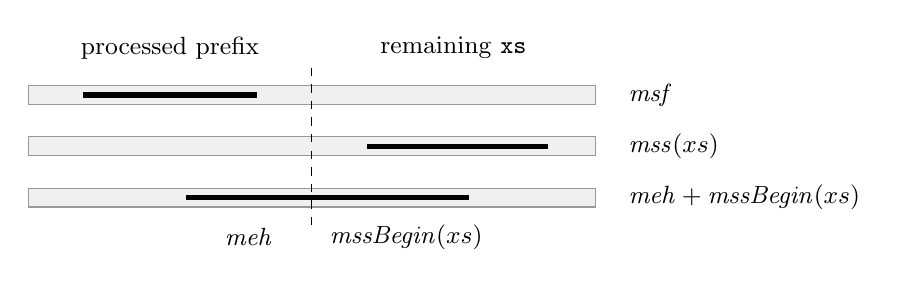
\begin{tikzpicture}[x=1cm,y=1cm,font=\small]
\node at (1.8,0.6) {processed prefix};
\node at (5.4,0.6) {remaining \code{xs}};
\foreach \y in {0,-0.65,-1.3} {
  \fill[black!6] (0,\y-0.12) rectangle (7.2,\y+0.12);
  \draw[black!40] (0,\y-0.12) rectangle (7.2,\y+0.12);
}
\draw[dashed] (3.6,0.35) -- (3.6,-1.65);
\draw[line width=2pt] (0.7,0) -- (2.9,0);
\node[anchor=west] at (7.5,0) {$\mathit{msf}$};
\draw[line width=2pt] (4.3,-0.65) -- (6.6,-0.65);
\node[anchor=west] at (7.5,-0.65) {$\mathit{mss}(xs)$};
\draw[line width=2pt] (2,-1.3) -- (5.6,-1.3);
\node[anchor=west] at (7.5,-1.3) {$\mathit{meh}+\mathit{mssBegin}(xs)$};
\node at (2.8,-1.8) {$\mathit{meh}$};
\node at (4.8,-1.8) {$\mathit{mssBegin}(xs)$};
\end{tikzpicture}
\caption{Three candidates for the maximum segment sum: within the processed
prefix, within the remaining suffix, or across the boundary. Segments may be
empty; each label gives the best sum for that case.}
\Description{Three copies of a list split at the same boundary. A highlighted
segment lies in the processed prefix, in the remaining suffix, or crosses the
boundary. The corresponding best sums are msf, mss xs, and meh plus mssBegin xs.}
\label{fig:kadane}
\end{figure}

Split the list into a processed prefix and the remaining suffix \code{xs}.
Figure~\ref{fig:kadane} shows the three possible locations of the best segment.
The crossing candidate combines the best suffix of the processed prefix
(\code{meh}) with the best prefix of \code{xs} (\code{mssBegin xs}).

For example, split \code{[1,-2,3,4,-1,2]} after the 4. The processed prefix has
$\mathit{meh}=7$ and $\mathit{msf}=7$, while the suffix has
$\mathit{mss}=2$ and $\mathit{mssBegin}=1$. The three candidates are 7, 2, and
$7+1=8$; the best segment crosses the boundary.
\begin{samepage}
So the invariant is
\[
  \mathit{kadaneHelper}(xs, \mathit{meh}, \mathit{msf})
  = \max\bigl(\mathit{msf},\ \mathit{mss}(xs),\ \mathit{meh} + \mathit{mssBegin}(xs)\bigr),
\]
under the preconditions that make the accumulators meaningful:
$\mathit{meh} \geq 0$ (the empty segment is always available) and
$\mathit{msf} \geq \mathit{meh}$ (the best segment so far is at least as good as
the best one ending here). Without the preconditions the statement is false: for
an empty \code{xs}, the right side would include $\mathit{meh}$ even when it
exceeds $\mathit{msf}$.
\end{samepage}

\subsection{The proof}

Once the invariant is written down, the proof is short:
\snippet*{kadaneCorrect}
The inductive step unfolds \code{kadaneHelper} once and applies the hypothesis
at the new accumulators. Here the hint is more specific than in the earlier
proofs: \code{ih `at` (Inst @"meh" meh', Inst @"msf" msf')} instantiates the
quantified accumulators explicitly. The solver could search for the
instantiation, but stating it makes the step easier and documents the argument.
The remaining equality between the instantiated hypothesis and the invariant
for \code{a .: as} is arithmetic over \code{smax}, which the solver checks
without further help, using the definitions of \code{mss} and \code{mssBegin}.
The preconditions are needed to instantiate the hypothesis: the new accumulators
satisfy them because \code{meh'} is a maximum with 0 and \code{msf'} is a
maximum with \code{meh'}.

The main theorem then follows by a calculation without induction. With both
accumulators 0, the invariant gives
$\max(0, \mathit{mss}(xs), \mathit{mssBegin}(xs))$, and the solver discharges the
last two steps: \code{mss} is nonnegative and at least \code{mssBegin} by its
definition. Abbreviated output shows the two results:
\begin{lstlisting}[style=output]
ghci> runTP kadaneCorrect
Inductive lemma: kadaneInvariant
  ...
  Result:                           Q.E.D.
Lemma: kadaneCorrect
  ...
  Result:                           Q.E.D.
\end{lstlisting}

\subsection{Lessons}

The effort in this proof went into one place: the invariant. Once we had
explained \emph{why} the algorithm works, as the three-way case analysis on where
the best segment lies, the mechanical checking was immediate. This division of
labor is typical of TP. The solver handles unfolding definitions, arithmetic,
and case analysis on \code{smax}; the human supplies generalizations and
intermediate statements. When a proof gets stuck, the useful question is
rarely ``which tactic is missing?'' and usually ``what is the statement that
explains this step?''

\begin{exercise}
\emph{Challenge.} Require the chosen segment to be nonempty. Write a
specification and a linear-time algorithm, and prove their equivalence under
an explicit nonempty-input precondition. Test all-negative lists.
Solutions: \code{mssNonEmpty}, \code{kadaneNonEmpty}, and
\code{kadaneNonEmpty\allowbreak Correct}. The independent segment enumerator is
\code{segmentNonEmpty\allowbreak Oracle}. The solutions return 0 on \code{[]}, outside the theorem's contract.
\end{exercise}

%==============================================================================
\section{Induction on decreasing measures}
\label{sec:datatype-induction}

The next two examples use \code{sInduct} to choose a measure suited to the
computation: the size of an expression tree, then the length of a search interval.

\subsection{Expression trees}

Return to \code{Expr}: mirroring swaps the children at every addition and
multiplication node, preserving evaluation because both operations commute.
\snippet{exprMirror}
Each binary case needs the hypothesis for both children before commutativity applies.
The calculational \code{induct} interface supports integers and lists, so for
this datatype we use \code{sInduct} with a size measure.
Reuse \code{exprSize} and its nonnegativity theorem \code{exprSizePos} from
Section~\ref{sec:mk-symbolic}. That theorem uses \code{inductiveLemma} to apply
the generated datatype induction principle without further guidance. Here
\code{exprSizeSmaller} uses this fact to show that each child is smaller than
its parent. These facts justify applying the hypothesis to each child.
The listing abbreviates the identical multiplication case; the companion
checks all three cases in full:
\snippet*{mirrorCorrect}
The hypothesis supplied by \code{sInduct} is conditional: it proves the result
for an expression only if its measure is smaller than that of the current
\code{e}. Each \code{smaller} hint discharges these conditions; the two
\code{ih} hints instantiate the hypothesis separately at \code{a} and \code{b}.
After substituting their evaluations, commutativity finishes the case.
The final \code{eval e} reconnects each binary case to the theorem's goal.
The \code{pCase} quasi-quoter splits the \emph{proof} by constructor and checks
that the cases cover the datatype; \code{sCase} defines symbolic functions.
The \code{Num} case has no recursive children and needs no hypothesis.
Running \code{runTP mirrorCorrect} checks all three cases and returns
\code{Proven}. The size argument is structural induction expressed through
\code{sInduct}'s more general principle of induction on a decreasing measure.

\subsection{Binary search with a decreasing interval}
\label{sec:binary-search}

Section~\ref{sec:midpoint} checked midpoint arithmetic. We now ask whether the
search itself finds a target in a sorted interval. SBV's
\code{TP.BinarySearch} example uses \code{Arr = SArray Integer Integer} and
\code{Idx = (SInteger, SInteger)}, with both bounds inclusive:
\libsnippet{binarySearch}
Here \code{sEDiv} by 2 computes the floor of the integer average, including for
negative bounds. The measure $\max(\mathit{hi}-\mathit{lo}+1,0)$ is the number
of indices remaining. On a nonempty interval, the midpoint lies within its
bounds, so either recursive call strictly decreases this measure. The empty
interval returns \code{sNothing}; a match returns \code{sJust mid}.

The companion imports this module as \code{Search} and
\code{Data.SBV.Maybe} as \code{SM}. We state the result contract explicitly:
\snippet*{binarySearchContract}
The predicate \code{Search.inArray} means that the target occurs at some index
between the bounds. If it occurs, \code{searchFound} requires a \code{Just}
result, an index within the interval, and the correct value at that index.
Otherwise the result must be \code{Nothing}. The theorem assumes that the array
is nondecreasing throughout the interval; duplicates are allowed, and no
particular matching index is prescribed.

The proof \code{binarySearchCorrect} uses \code{sInduct} with the same interval
measure. Its two helper lemmas show that restricting the search to the selected
half preserves sortedness and whether the target occurs. In the upper-half
case, for example, all values at or below the midpoint are too small. The
calculation supplies that range lemma and instantiates the induction hypothesis
at $[\mathit{mid}+1,\mathit{hi}]$; the lower-half case is symmetric. Empty
intervals and immediate matches close directly. Running
\code{binarySearchProof} checks this argument with CVC5, including termination
of \code{bsearch}; the complete calculation is in the companion.

This proof uses unbounded integer indices, so \code{lo + hi} cannot overflow.
It complements the earlier arithmetic proof, but does not verify a fixed-width
implementation of the whole search: that further step must also justify the
index conversions and updates \code{mid+1} and \code{mid-1}.

%==============================================================================

\section{Failed TP proofs and counterexamples}
\label{sec:tp-failures}

A failed TP run is a diagnostic about an obligation, not a verdict on every
statement in the script. A solver can refute the stated theorem, refute an
intermediate equality, or leave an obligation unresolved. The examples below
make these outcomes concrete; the companion runs the expected failures and
checks their diagnostics. The first example adapts
\code{Documentation.SBV.Examples.TP.Basics}.

\subsection{Concrete inputs and observed values}

Suppose a length function returns 42 whenever its input has more than five
elements and contains 42. This intentionally incorrect definition is compared
with the library length function:
\snippet{badLengthProof}
\code{observe} names expressions to include in the model; it does not add a
premise to the theorem. Running \code{runTPWith z3Timeout5 badLengthProof}
produces the following diagnostic in our validation run, followed by a
\code{Failed} exception:
\begin{lstlisting}[style=output]
Lemma: badLengthProof
*** Failed to prove badLengthProof.
Falsifiable. Counter-example:
  xs   = [11,13,16,18,21,42] :: [Integer]
  imp  =                  42 :: Integer
  spec =                   6 :: Integer
\end{lstlisting}
The universal input \code{xs} has become a concrete finite list. The observations
explain the disagreement: the implementation returns 42, while the specification
returns 6. The elements other than 42 have no particular significance; another
solver run may choose different ones. Evaluate both sides on the reported input
before deciding whether the implementation or the specification needs repair.
Validation checks the displayed model with ordinary list length and membership.
TP does not return a \code{Proof} for a refuted obligation. Its validation driver
catches the exception because failure is expected in this example.

\subsection{A failed step in a true theorem}

A calculation can fail even when its advertised theorem is true:
\snippet{badCalculation}
The theorem is the identity $n+n=2n$, but the first step incorrectly inserts 1.
For \code{runTPWith z3Timeout5 badCalculation}, the relevant output is:
\begin{lstlisting}[style=output]
*** Failed to prove badCalculation.1.
Falsifiable. Counter-example:
  n = 0 :: Integer
\end{lstlisting}
This refutes the first equality, $n+n=2n+1$: its two sides are 0 and 1 at the
reported input. It does not refute $n+n=2n$, which the companion proves separately.
The suffix \code{.1} identifies the failing obligation. Remove the incorrect
step and the calculation can establish its intended theorem.

More generally, the model satisfies the assumptions and hints available to that
step and falsifies its goal. A missing premise, a missing lemma, or an induction
hypothesis instantiated at the wrong arguments can leave an obligation too weak.
A model of such an obligation need not describe a reachable program execution.
Inspect the local goal and its premises before treating it as a bug in the
original program. Conversely, a timeout or \code{unknown} supplies no refuting
model: the \code{revWeak} attempt in Section~\ref{sec:induction} is unresolved,
not disproved. Termination-check failures concern admissibility of a definition
and are a further, separate diagnostic (Section~\ref{sec:termination}).

\subsection{An incorrect justification}
\label{sec:bad-hint}

A Boolean expression supplied with \code{??} is itself a proof obligation.
SBV first checks that it follows from the local assumptions, before using it to
justify the equality. For example, the following calculation inserts the
unjustified claim that its arbitrary integer input is nonnegative:
\snippet{badJustification}
Both the stated theorem and the equality are valid, but the hint is not.
To see the separate check of Boolean hints, enable \code{printAsms}:
\snippet{showHintFailure}
Running \code{showHintFailure} produces:
\begin{lstlisting}[style=output]
Lemma: badJustification
  Asms: 1
*** Failed to prove assumptions for badJustification.1.
Falsifiable. Counter-example:
  n = -1 :: Integer
\end{lstlisting}
At this input the proposed justification is false, although the equality still
holds: both sides are $-2$. The words \emph{assumptions for} distinguish this
failure from a refuted calculation step. Here the repair is simply to remove
the hint. If a proof genuinely needs a nonnegative input, that restriction must
be justified by the surrounding context or made a precondition of the theorem;
inserting it with \code{??} does not establish it. Unlike a previously proved
lemma supplied as a hint, a fresh Boolean hint must be discharged at its point
of use. In the pinned SBV version these checks are normally quiet, including
their failure diagnostics; \code{printAsms = True} exposes the counterexample.
Validation checks that the reported integer refutes the hint while satisfying
the equality.

\subsection{Function interpretations as counterexamples}

A model can also describe an uninterpreted operation. The library example
\code{forall\allowbreak Disjunction\allowbreak Not} attempts the invalid equivalence
\[
 ((\forall x.\ p(x))\lor(\forall x.\ q(x)))
 \quad\Longleftrightarrow\quad \forall x.\ (p(x)\lor q(x)).
\]
With \code{p} and \code{q} uninterpreted predicates on integers, TP reports:
\begin{lstlisting}[style=output]
p :: Integer -> Bool
p 3 = True
p _ = False

q :: Integer -> Bool
q 3 = False
q _ = True
\end{lstlisting}
These are finite descriptions of total functions: the underscore gives the
value at every unlisted input. At each integer at least one predicate is true,
but neither predicate is true at every integer. Thus the right side holds and
the left side fails. The exceptional integer need not be 3 in another run.
The companion invokes the library example and checks this interpretation of its
model. Models of functions, arrays, and datatypes should be read according to
their symbolic domains, just as scalar counterexamples are.


\section{Polymorphic and higher-order proofs}
\label{sec:higherorder}

Proof scripts can be reused across types and parameterized by operations.
The next examples show what each form of reuse establishes.

\subsection{Polymorphic scripts, monomorphic proofs}
\label{sec:polymorphic}

Reversal preserves length regardless of the element type. We can express the
proof once, using Haskell polymorphism:
\snippet*{reverseLength}
The Haskell \code{forall a} makes the \emph{script} polymorphic; \code{SymVal a}
provides the symbolic representation of its elements. Before running it, we
choose a monotype. For example, in GHCi:
\begin{lstlisting}
runTP (reverseLength @Integer)
runTP (reverseLength @Word8)
\end{lstlisting}
Each invocation checks a separate theorem over that type's solver sort. The
companion runs both.

This differs from \code{Forall "xs" [a]}, which quantifies over \emph{values}
inside the theorem after \code{a} has been chosen. A successful integer instance
does not by itself certify every type instance of the script: SBV is not
quantifying over Haskell types. Polymorphism lets us reuse the argument and its
implementation, while each proof run establishes a monomorphic result. This
distinction matters especially for arithmetic laws, whose truth may change
between \code{Integer} and \code{Word8}.

%==============================================================================
\subsection{The bookkeeping law}

Many useful list laws concern an operation supplied by the caller. The
\emph{bookkeeping law}, adapted here from
\code{Documentation.SBV.Examples.TP.Lists}, says that reducing a concatenation
equals reducing each chunk and then reducing those results:
\[
 \mathit{reduce}(\mathit{concat}\ xss)
 = \mathit{reduce}(\mathit{map}\ \mathit{reduce}\ xss),
 \qquad \mathit{reduce}=\mathit{foldr}\ f\ e.
\]
Associativity of $f$ and a two-sided identity $e$ suffice. For integer addition
with identity 0, this is ``sum the elements'' versus ``sum the chunk sums.''
Commutativity is not assumed: the order of elements is preserved.
Both the outer list \code{xss} and every chunk are finite; the law makes no
claim about consuming an infinite stream of chunks.



We reuse a library lemma with the following import:
\snippet{listProofImports}
The proof has two dependencies: \code{foldrOverAppend}, and a helper
\code{foldBase} proved in the companion. Their conclusions are, respectively,
\[
\begin{aligned}
 \mathit{foldr}\ f\ e\ (xs \mathbin{++} ys)
   &= \mathit{foldr}\ f\ (\mathit{foldr}\ f\ e\ ys)\ xs,\\
 \mathit{foldr}\ f\ y\ xs &= f\ (\mathit{foldr}\ f\ e\ xs)\ y.
\end{aligned}
\]
The first needs no assumptions on $f$. The second requires associativity and
the left-identity law. Its empty-list case uses
$f\ e\ y=y$; its inductive step uses associativity to move $y$ past the head.
These lemmas expose exactly the two transformations the main induction needs:
\snippet*{bookKeeping}
\code{quantifiedBool} packages a quantified property as an \code{SBool}, so the
algebraic laws can appear as assumptions in the calculation and as the premise
of the theorem. They are not unconditionally added as user axioms. Induction
is over the outer list of chunks: unfold \code{concat}, move the fold across
append, use the induction hypothesis on the remaining chunks, then use
\code{foldBase} to combine their result with that of the first chunk.

The left-identity assumption has a concrete purpose. Take $f\ x\ y=x$ and
$e=0$. This operation is associative and has right identity 0, but for
\code{xss = [[],[1]]}, the two sides of the bookkeeping law are 1 and 0.
The empty first chunk contributes an identity that must work on the left.
The companion checks this counterexample as well as the proof.

\subsection{An arbitrary operation at a fixed type}

The parameters \code{e} and \code{f} are Haskell arguments to the proof script.
To prove the law without choosing an implementation of the operation, give
them fresh uninterpreted names:
\snippet{bookKeepingRun}
An \code{uninterpret} declaration supplies a logical name without defining
equations. Here \code{combine} is a total function on integers; the proof must
work for every interpretation satisfying the stated algebraic laws. The solver
does not enumerate implementations of \code{combine}. SBV specializes its list
operations to this logical operation and reasons about the resulting
definitions. The higher-order Haskell interface thus supports a proof about an
arbitrary operation at a fixed type. We do not pass a Haskell function as an
ordinary \code{Forall} argument of the theorem.

Passing \code{0} and \code{(+)} instead gives a concrete instance. The companion
also checks that instance and derives the unconditional sum-of-chunk-sums law.
An uninterpreted operation represents a total mathematical function; it does
not model divergence or exceptions in a Haskell callback.

\subsection{Closures and higher-order functions}
\label{sec:closures}

Ordinary Haskell allows \code{map (+k) xs}; \code{SL.map (+k) xs} needs an
explicit \code{Closure} when \code{k} is a symbolic unknown from the enclosing
solver context:
\snippet{closure}
SBV passes \code{k} through the recursion as \code{env}, so \code{closureFun}
need not capture it. Literals and globally named logical symbols need no such
environment. The companion proves length preservation for every offset and
finite integer list.

%==============================================================================
\section{A verified tautology checker}
\label{sec:tautology}

The checker in this section is a small verified decision procedure for
propositional logic. It accepts a finite formula exactly when the formula is
true under every assignment, and it can produce a falsifying assignment when
the answer is no. Its design follows a classic development by
\citet[Chapter~4]{boyermoore}, later formalized in Imandra~\citep{imandraTautology}.
The SBV development is
\code{Documentation.\allowbreak SBV.\allowbreak Examples.\allowbreak TP.\allowbreak TautologyChecker}.
We follow the algorithm and its main proof obligations; listings below are
extracted from that module, with whitespace adjusted in the longer declarations.
The companion imports it qualified as \code{Taut}.

\subsection{Formulas, assignments, and evaluation}

A formula is a constant, a variable identified by an integer, or a conditional:
\libsnippet{tautFormula}
Conditionals suffice to encode the familiar connectives. Writing $p$ and $q$
for formulas, negation is \code{If p FFalse FTrue}, conjunction is
\code{If p q FFalse}, and implication is \code{If p q FTrue}. These are formulas
of the object language; \code{If} constructs a formula rather than evaluating
a Haskell conditional.

An assignment is a list of \code{Binding} values, each pairing a variable ID
with a Boolean. \code{lookUp} uses the first matching binding and defaults to
false if none is present. Evaluation is structural recursion:
\libsnippet{tautEval}
This gives the specification independently of the checking algorithm. A tautology
must evaluate to true for \emph{every} assignment, not just the empty assignment.
Defaults make evaluation total; they do not mean that a variable is fixed to
false when asking whether a formula is a tautology. Every assignment to the
finitely many variables of a formula can be represented by a finite binding list.

We will follow two examples: $p\Rightarrow p$, represented by
\code{If (Var 0) (Var 0) FTrue}, and $p\Rightarrow q$, represented by
\code{If (Var 0) (Var 1) FTrue}. The first is a tautology. The second is false
when variable 0 is true and variable 1 is false.

\subsection{Normalization and a decreasing measure}

The checking traversal expects a normal form in which the condition of every
\code{If} is a constant or a variable. A conditional can occur in either branch,
but not as another conditional's condition. Normalization repeatedly distributes
a nested condition:
\[
 \mathit{If}\ (\mathit{If}\ p\ q\ r)\ l\ r'
 \quad\longmapsto\quad
 \mathit{If}\ p\ (\mathit{If}\ q\ l\ r')\ (\mathit{If}\ r\ l\ r').
\]
If $p$ is true, both sides choose between $l$ and $r'$ using $q$; otherwise they
use $r$. The rewrite therefore preserves meaning. For example, the condition of
$(p\land q)\Rightarrow q$ is initially an \code{If}; this rewrite exposes $p$
as the outer test. The complete definition supplies both the measure and its
supporting lemmas:
\libsnippet*{tautNormalize}
Termination is not structural: the first branch can produce a larger tree by
duplicating $l$ and $r'$. The supplied measure is a lexicographically ordered
pair. Write $C$ for \code{ifComplexity} and $D$ for \code{ifDepth}. On constants
and variables, $C=1$ and $D=0$; on conditionals,
\[
 C(\mathit{If}\ c\ l\ r)=C(c)\bigl(C(l)+C(r)\bigr),
 \qquad D(\mathit{If}\ c\ l\ r)=1+D(c).
\]
The distributive rewrite preserves $C$ and reduces $D$ by one. Recursing into
either branch of an ordinary conditional strictly reduces $C$, since every
complexity is positive. Each call therefore decreases the pair even when tree
size increases. Proved facts supplied through \code{measureLemma} justify these
checks. Separate lemmas establish that normalization produces a normal formula
and preserves its evaluation under every assignment.

\subsection{Checking both branches consistently}

The worker maintains bindings for variables already tested along the current
path. Here is the complete traversal:
\libsnippet*{tautCheck}
Constants settle immediately. At an \code{If} whose condition is a known
variable, the worker follows the branch fixed by its binding. For an unassigned
variable it checks both branches, prepending a true binding for the left branch
and a false binding for the right. Repeated occurrences must respect the same
choice: they are not independent Boolean inputs. A bare variable is accepted
only when its lookup is true; an unassigned bare variable is correctly rejected
because choosing it false is a counterexample. The final case rejects a nested
condition, which normalization rules out before the traversal starts:
\libsnippet{tautTop}

For $p\Rightarrow p$, the first test splits into two cases:
\begin{center}
\begin{tabular}{lll}
\toprule
Path assumption & Remaining formula & Result \\
\midrule
$p=\mathit{True}$  & $p$                & true by lookup \\
$p=\mathit{False}$ & $\mathit{FTrue}$   & true immediately \\
\bottomrule
\end{tabular}
\end{center}
Both paths succeed. For $p\Rightarrow q$, the true branch reaches the unassigned
variable $q$ and fails; the false branch still succeeds. The conjunction of the
two results is false. This is a search through consistent assignments, with
branches pruned when a variable already has a value; it can still explore
exponentially many cases.

The companion checks these examples and 70 formulas in total against an
independent Haskell evaluator and all four assignments to variables 0 and 1.
The collection includes nested conditions, so it also checks normalization and
its truth preservation. These finite checks illustrate the algorithm; the
following proofs establish the universal claims.

\subsection{Soundness through a generalized invariant}

The key lemma does not start with an empty environment. For every formula $f$,
path bindings $b$, and further bindings $a$, it establishes
\[
 \mathit{isNormal}\ f\ \land\ \mathit{isTautology'}\ f\ b
 \quad\Longrightarrow\quad \mathit{eval}\ f\ (b\mathbin{++}a).
\]
The leading bindings $b$ retain priority over the arbitrary completion $a$.
This generalization is essential: recursive calls extend $b$, so a hypothesis
only about the empty environment would not apply. It is the same design move
used for the accumulator in reversal and Kadane's invariant.

The proof uses \code{sInduct} with \code{ifComplexity}. In the unassigned-variable
case, checking has established both branch results, one with the variable true
and one with it false. Split on that variable's value in the arbitrary
completion. Apply the induction hypothesis to the corresponding branch and
use the binding lemmas to show that its extended environment agrees with the
original evaluation. When the variable is already assigned, only its selected
branch matters. Positivity and branch-decrease lemmas discharge the measure
obligations. This isolates three groups of reusable facts: lookup under extension,
normalization, and correctness of the traversal under path assumptions.

The top-level soundness calculation assembles those facts:
\libsnippet*{tautSoundness}
First, \code{normalizeRespectsTruth} replaces evaluation of the original formula
by evaluation of its normalization. Then \code{normalizeCorrect} supplies the
normal-form premise, and \code{tautologyImpliesEval} is instantiated with empty
path bindings and the arbitrary input assignment. The conclusion is true.
The theorem covers every finite formula and every finite binding list; it is
not limited to the formulas used in the concrete tests.

\subsection{Completeness and a falsifying assignment}

Rejection should also have a meaning. The function \code{falsify} normalizes
its input and traverses it with bindings, like the checker, but seeks one
failing path rather than requiring both paths to succeed. Its result records
whether a counterexample was found and a list of bindings. A false constant
returns the current bindings; an unassigned variable can be made false. At a
new conditional test, the search tries the true branch and tries the false
branch if the first attempt finds no counterexample.

For $p\Rightarrow q$, this produces $p=\mathit{True},q=\mathit{False}$.
Evaluating the \emph{original} formula under that assignment gives false. The
completeness theorem establishes this behavior for every rejected formula:
\libsnippet{tautCompleteness}
The helper theorem establishes falsification of the normalized formula; truth
preservation transfers that result back to the original input. Combined with
soundness, rejection has a concrete witness and acceptance holds under every
assignment. The returned bindings are produced by our verified traversal,
whereas the counterexamples in Section~\ref{sec:tp-failures} are models supplied
by the SMT solver when it refutes a proof obligation.

The companion runs both top-level proofs and their dependencies, with some
obligations using CVC5. The proof structure follows the program structure:
small lemmas establish lookup and normalization facts, a generalized induction
handles the traversal, and short final arguments expose the public guarantees.
This makes a verified algorithm understandable without reproducing every helper
proof in the tutorial.

%==============================================================================


\outlinepart{IV. Boundaries and context}
\section{C generation from verified functions}
\label{sec:codegen}

\subsection{A verified function across the translation boundary}

A theorem about a symbolic function and a claim about an executable program
meet at a translation boundary. To make that boundary concrete, we return to
the first specification in the tutorial. SBV translates a symbolic function to
C code that runs without a solver. For the saturating adder
of Section~\ref{sec:specs}:
\snippet{codegen}
This produces \code{sat\_add.c} and a matching header. Because the C code is
generated from the same \code{satAdd} that we proved correct, there is no manual
rewrite in which the two could drift apart. For this adder, the generated header
maps \code{SWord8} to \code{uint8\_t}, and the arithmetic helpers implement
8-bit modular addition and subtraction using unsigned intermediates and masks.

\subsection{Executable validation and trust assumptions}

The companion checks the compiled artifact exhaustively: it compiles the
generated adder with undefined-behavior sanitization and compares all 65,536
inputs with an independent oracle written directly in C. This checks the
translation and compilation boundary for the generated executable;
Section~\ref{sec:pitfalls} explains the remaining trust assumptions.

Not all of SBV's vocabulary is executable. Quantifiers and uninterpreted sorts,
for example, have no operational meaning, and the code generator rejects programs
that use them rather than approximating them. Uninterpreted functions become calls
to C functions that the user provides, which then join the trusted code.

%==============================================================================
\section{The execution model and its proof obligations}
\label{sec:hood}

Two questions connect the examples to their implementation: what does Haskell
evaluate before the solver runs, and which definitions may the proof rely on?
The representation of symbolic values explains the first; termination and the
choice of a finite, total domain explain the second. These distinctions help
predict both the cost of constructing a query and the scope of its answer.

\paragraph{Symbolic values are deferred graph nodes.}
Internally, a value of type \code{SBV a} is either a concrete constant or a
deferred computation that, given the state of the current symbolic run, adds a
node to a graph and returns its identifier:
\begin{lstlisting}
newtype SBV a = SBV SVal
data SVal     = SVal Kind (Either CV (Cached SV))
newtype Cached a = Cached (State -> IO a)
\end{lstlisting}
The addition function \code{\textbackslash{}x y -> x + y} can therefore have
the pure type \code{SWord8 -> SWord8 -> SWord8} and still allocate graph nodes. Operations
on constants are folded immediately, which is why \code{satAdd 250 10} evaluates
to \code{255} without a solver. The run-time \code{Kind} records the logical sort,
so simplifications can respect it: rewriting \code{x .== x} to true is valid for
integers but not for floats.

\paragraph{Sharing comes in two forms.}
A generator that combines a term with itself, such as
\code{iterate (\textbackslash{}t -> t + t) x !! 30}, describes a term that is
exponentially large as a tree but linear as a graph. SBV preserves this sharing
in two ways. It memoizes each deferred computation, using stable names in the
style of observable sharing~\citep{sharing}, so that forcing the same Haskell
value twice yields the same node. It also interns nodes, so that separately
constructed applications of the same operator to the same arguments reuse a node.
Neither mechanism identifies arbitrary mathematically equal expressions.

\paragraph{Nodes belong to a run.}
A graph node is meaningful only in the run that created it. Two values of type
\code{SInteger} from different calls to \code{prove} cannot be combined, even
though their types agree, and SBV checks for common mistakes of this kind. To
carry a result from one run to another, extract a concrete value from a model
and turn it back into a literal. Section~\ref{sec:queries} illustrates the same
concrete-to-symbolic conversion with \code{literal v}, though its loop stays
within one run. Constants and reusable function definitions can be shared
across runs; session-specific symbolic unknowns cannot.

\paragraph{Queries synchronize dependencies.}
When a query creates a new term, SBV records the declarations it requires: sorts
for datatypes (including those nested inside lists, tuples, or other datatypes),
uninterpreted constants, and definitions of \code{smtFunction}s it calls. Before
the term is used, any of these that the solver has not seen are sent. This is why
a datatype can first appear inside a query. The companion exercises this case
with two fresh values of a parameterized datatype created by \code{freshVar}.

\subsection{Termination is a proof obligation}
\label{sec:termination}

SMT functions denote total functions. An equation such as $b(n)=b(n)+1$ has
no integer-valued solution; admitting it as a definition would make the logical
context inconsistent and allow unrelated claims to be proved. TP therefore
checks termination of the symbolic functions used in a proof, separately from
checking the theorem itself.

SBV tries automatic measures such as list length or datatype size. For recursion
on a list's tail, length decreases at each call and is bounded below by zero,
so the calls cannot continue indefinitely. The
\code{Functions proven terminating} line reports these checks. If the automatic
check fails, supply a measure with \code{smtFunctionWithMeasure}; the normalizer
in Section~\ref{sec:tautology} illustrates a lexicographic measure. An unknown
solver result does not establish termination. Explicitly bypassing a check with
\code{smtFunctionNoTermination} leaves a dependency reported as \code{Modulo}
the function's termination. The companion checks that $b(n)=b(n)+1$ is rejected.

\subsection{Finite lists and datatypes}
\label{sec:finite-lists}

Symbolic lists and recursive algebraic datatypes contain finite, total values:
no undefined elements, partial tails, or infinite constructor trees. Sizes are
unbounded, but each value is finite. For example, double reversal is the identity
on finite lists, while for \code{xs = repeat 0}, \code{take 1 xs} returns
\code{[0]} and \code{take 1 (reverse (reverse xs))} diverges. This domain makes
structural induction and decreasing-size arguments available; total reasoning
and its relationship to partial languages are studied by
\citet{fastloose}. Arrays instead denote total mappings over possibly infinite
index domains (Section~\ref{sec:arrays}); they do not introduce infinite recursive
constructor structure.

%==============================================================================
\section{Proof results, diagnostics, and trust}
\label{sec:pitfalls}

\subsection{Failed checks and diagnostic steps}
\label{sec:troubleshooting}

Before proving, run \code{testSatAdd} to check \code{satAddSpec} on random byte
inputs with \code{sbvQuickCheck}. The companion checks this result before proving;
passing random tests is not a proof.

Pass \code{"sat-add.smt2"} to this helper to inspect solver commands:
\snippet{inspectSatAdd}
Here \code{verbose} prints abbreviated diagnostics; \code{transcript} writes
SMT-LIB. Replay it outside GHCi with \code{z3 sat-add.smt2}.

\begin{description}
\item[The solver cannot start.] Run \code{z3 --version} in the same shell and
  check that the executable is on \code{PATH}. Installing SBV does not install Z3.
\item[The solver returns unknown or times out.] No conclusion follows.
  Simplify the obligation and check whether its theories suit the solver;
  nonlinear arithmetic is a common obstacle. Use \code{z3Timeout5} from
  Section~\ref{sec:host} to bound each solver call to 5,000 milliseconds.
  \code{SetTimeOut} does not limit the whole TP run, which may make many calls.
\item[A counterexample is found.] Evaluate implementation and specification on
  that input. The result of \code{wrongAdd 223 124} is 91. The specification
  evaluates \code{min 255 (223 + 124 :: Integer)} to 255, which agrees with
  the corrected \code{satAdd}. Check which side disagrees with the intended behavior.
\item[A TP calculation stalls.] Find the failed step and distinguish a
  counterexample from unknown. Check its assumptions and the \code{??} hints
  on that equality, instantiate hypotheses explicitly, or split the step with
  an intermediate expression. If the recursive call changes an accumulator,
  generalize the statement as in Sections~\ref{sec:induction} and~\ref{sec:kadane}.
  Section~\ref{sec:tp-failures} shows concrete TP diagnostics and how to interpret
  the models of failed obligations.
\end{description}

\paragraph{Common pitfalls.}
\begin{itemize}
\item \emph{Wrong domain.} A property proved over \code{SInteger} says nothing
  about \code{SInt32}, and vice versa. Choose the type that matches the code you
  care about. List and recursive-datatype theorems cover finite, total values only
  (Section~\ref{sec:finite-lists}).
\item \emph{Specification repeats the implementation.} Write specifications in a
  different style or a wider domain (Section~\ref{sec:specs}).
\item \emph{Haskell \code{if} or recursion on symbolic data.} Use \code{ite} and
  \code{sCase} for symbolic choices, and \code{smtFunction} for recursion over
  symbolic structure (Section~\ref{sec:host}).
\item \emph{Contradictory assumptions.} If \code{constrain}ed assumptions are
  unsatisfiable, everything is provable. A quick \code{sat} on the assumptions
  alone detects this.
\item \emph{Mixing runs.} Unknowns belong to the run that created
them; move concrete values instead (Section~\ref{sec:hood}).
\end{itemize}

\paragraph{What a proof rests on.}
A Q.E.D. from SBV depends on the correctness of SBV's translation to SMT-LIB, the
solver, and, for TP, the generation of proof obligations. TP proofs also depend on
any axioms the user introduces and on any functions whose termination checks
were explicitly bypassed. SBV tracks these dependencies: a proof that rests on an
axiom, or on an unfinished step marked with \code{sorry}, is reported as
\code{Modulo} the offending lemmas rather than as \code{Proven}. TP does not replay solver certificates in an independent proof
kernel. Functional correctness does not establish running-time or space bounds.
For generated C, the C compiler and code generator join the trusted base:
Section~\ref{sec:codegen}'s exhaustive check covers the tested executable and
input domain, rather than verifying either compiler in general.

%==============================================================================



\subsection{Encodings and solver selection}
\label{sec:encodings-and-solvers}

Solver selection starts with the meaning of the formula. Integer addition and
byte addition are not interchangeable encodings of the same operation unless
the relationship is stated. For example, this bridge theorem relates modular
byte addition to an integer expression:
\snippet{encodingBridge}
\code{prove byteAdditionBridge} checks the connection rather than assuming it.
If an abstraction omits the modulus, it needs a no-overflow precondition.
Similarly, replacing a finite list by an integer-indexed array introduces a
total memory model; length and bounds must be carried separately.

After fixing semantics, compare formulations by inspecting the emitted problem
and measuring the actual obligations. A finite Boolean circuit, quantified
integer formula, and recursive sequence definition expose different work to a
solver. No universal ranking of backends follows. The companion checks the byte
field theorem with both \code{proveWith z3 fieldRoundTrip} and
\code{proveWith cvc5 fieldRoundTrip}; changing the backend does not change the
intended statement, but support and effectiveness depend on the theories used.
Optimization remains a Z3-specific SBV interface in this tutorial.

When a formulation stalls, first identify whether the difficulty is recursion,
quantifier instantiation, nonlinear arithmetic, or the size of a finite encoding.
Then try a justified reformulation or supply a lemma. Keep the model and its
oracle unchanged while comparing attempts, preserve timeouts, and record solver
versions and transcripts. A faster answer to a weakened property is not a
successful optimization of the proof task.


\subsection{Model validation and proof dependencies}
\label{sec:proof-audits}

A printed \code{Q.E.D.} is only part of the report. TP also records dependencies,
including unproved steps and user axioms. The following deliberately checks the
same true identity twice, once normally and once with \code{sorry} supplied:
\snippet*{auditProofs}
The normal proof has \code{RootOfTrust Nothing}; the draft has a nonempty root
of trust and is displayed as \code{Modulo: sorry}. The dependency tree shows the
path from \code{draftIdentity} to \code{sorry}. This remains a draft even though
its statement happens to be true. Removing the placeholder and rerunning the
proof is what establishes the checked version.

\code{showProofTree True} compresses repeated uses of a dependency; use
\code{False} to retain them. \code{rootOfTrust} identifies the outstanding
trusted dependencies. \code{axiom} introduces a proposition without proving it,
and bypassing a function's termination check creates another trust dependency.
These are different from explicit premises of a conditional theorem, whose
logical role is visible in the statement. Inspect both the theorem and its
root of trust before reusing it.

For refutations, audit the witness as well. Re-evaluate concrete inputs with an
independent interpreter or arithmetic calculation, check function defaults and
array updates, and distinguish a local proof-step model from a program input.
The validation driver does this for the examples in Section~\ref{sec:tp-failures}.
For successful checks, dependencies explain what was assumed; they do not
replace the solver and translation components of the trusted base described
above. Keep the checked source, solver configuration, and validation record
together so the claim remains reproducible.


\section{Connections to program reasoning}
\label{sec:related}

The examples place SBV within a broader set of approaches to reasoning about
functional programs. Three questions make the connections useful: how is the
program represented, how is a proof decomposed, and what does a successful check
establish?

\subsection{Testing and symbolic evaluation}

QuickCheck~\citep{quickcheck} treats a property as an executable function and
searches for counterexamples by sampling inputs. Symbolic reasoning instead
represents unknown inputs and asks whether a violating assignment exists.
For \code{satAddSpec}, the independent specification serves both purposes:
Section~\ref{sec:troubleshooting} tests it before asking the solver to prove it.
The practical connection is a shared specification and concrete feedback, while
the evidence differs: successful tests cover the executed inputs, and an
unsatisfiability result rules out a counterexample throughout the modeled domain.

Rosette~\citep{rosette} develops solver-aided host languages using a symbolic
virtual machine, demonstrated in Racket. Grisette~\citep{grisette} brings
symbolic evaluation and state merging to Haskell as a library;
Smten~\citep{smten} translates high-level symbolic computations in a
Haskell-derived language to SMT queries. These approaches address a common
representation problem: execution with unknown data must preserve the possible
outcomes of symbolic choices. In our examples, \code{ite} and \code{sCase}
make those choices explicit, while ordinary Haskell computes the query generator.
The what4 library~\citep{what4} provides typed symbolic values and solver
interfaces for building verification tools. SBV's interface combines symbolic
programming, model extraction, and explicit proof calculations in one library.

\subsection{Equational reasoning and proof guidance}
\label{sec:related-calculation}

\citet{danvyfoldunfold} teaches equational reasoning about recursive programs in
Coq using fold--unfold lemmas. A recursive definition supplies equations for its
constructor cases, and controlled rewriting makes their use visible in a proof.
Our mirror calculation illustrates a related teaching choice: unfold the
transformation, apply the hypotheses for both children, and then use
commutativity. The displayed steps explain the argument even when automation
could combine several of them. The checking mechanisms differ: our \code{=:}
links generate SMT obligations, and hints provide facts for the following link.

The expression evaluator also connects to tutorials on programming-language
semantics. \citet{huttonsemantics} uses a minimal arithmetic language to develop
semantic descriptions and calculate an abstract machine. Our evaluator serves
as the specification of a transformation: \code{mirrorCorrect} proves that
changing syntax preserves meaning. Reusing \code{Expr} for search and proof
lets the reader see the change from finding one term with a desired evaluation
to establishing an equation for every finite term.

Generalization is the crucial step when the computation carries extra state.
The reversal proof needs a statement about an arbitrary accumulator because a
recursive call changes it; Kadane's proof needs an invariant describing the
remaining suffix under arbitrary admissible accumulator values. In each case,
the stronger statement makes the induction step possible. This is the reusable
lesson of the calculations, independently of their concrete proof notation.

\subsection{Refinements, invariants, and the scope of a proof}

Liquid Haskell~\citep{liquidhaskell} adds logical refinements to Haskell types.
Refinement reflection~\citep{reflection} makes function definitions available
to the refinement logic and supports equational proofs written as Haskell
programs, with pattern matching and recursion expressing case splits and
induction. It therefore shares our interest in combining user-written proof
structure with SMT reasoning. The interface differs: Liquid Haskell checks
refinements of Haskell programs, while our SBV scripts construct symbolic
models and execute TP checks. A \code{Proof} value is obtained by running those
checks; ordinary GHC typechecking of a script does not establish its theorem.

Dafny~\citep{dafny} provides a language and verifier in which programmers supply
specifications and invariants and the verifier uses SMT to discharge the
resulting obligations. The accumulator invariant in our Kadane development
plays a comparable explanatory role: it describes what remains true as the
state changes, here across recursive calls rather than an imperative loop.

For readers moving between these approaches, it is useful to carry over the
specification and the mathematical argument before translating the notation.
Check which numeric domains, termination conditions, and notions of equality
the target system uses. Our finite-data scope (Section~\ref{sec:finite-lists})
and monomorphic theorem instances (Section~\ref{sec:polymorphic}) are part of the
claim being proved, not incidental details of the proof script.

%==============================================================================
\section{Suggested projects}
\label{sec:projects}

\subsection{Project: from recursive invariants to state transitions}
\label{sec:stateful-programs}

Transfer the invariant-discovery method from Kadane's algorithm to a program
represented by successive states. Begin with integer state $(x,y)=(1,1)$ and
the simultaneous update
\[
 (x,y)\longmapsto(x+1,y+x).
\]
The safety property is $y\geq1$ after any number of steps. Work through the
following stages; this is an open-ended project rather than an additional
worked solution in the companion.
\begin{enumerate}
\item Encode the initial state, transition relation, and unsafe states. Search
  for an execution reaching $y<1$ within a chosen bound. Explain why finding no
  such execution establishes safety only up to that bound.
\item Try to prove that $y\geq1$ holds initially and is preserved by every
  transition from a state satisfying it. Inspect a counterexample to preservation
  and decide whether it is reachable from $(1,1)$.
\item Strengthen the invariant so that both initialization and preservation can
  be proved. Explain why the strengthened invariant establishes safety at every
  finite depth, and compare this strengthening with generalizing the accumulator
  hypothesis in Section~\ref{sec:kadane}.
\item As an extension, express a bounded loop performing the updates using the
  weakest-precondition interface. Separate its safety assertion from the extra
  argument needed to establish termination.
\end{enumerate}

\paragraph{Starting hints.}
Use mathematical integers first, so overflow does not change the question.
The next value of $y$ depends on $x$; a lower bound on $x$ may therefore be
needed even though the requested safety property mentions only $y$.
For example, $(-1,1)\longmapsto(0,0)$ refutes preservation of $y\geq1$ alone,
but is not an execution starting from the specified initial state. A
counterexample to inductiveness is an invitation to inspect the invariant,
not automatically a counterexample to safety.

For starting code, see these modules under
\code{Documentation.\allowbreak SBV.\allowbreak Examples}:
\begin{itemize}
\item \code{ProofTools.\allowbreak BMC} demonstrates bounded reachability with
  a state datatype and a transition relation.
\item \code{ProofTools.\allowbreak Strengthen} contains this update and
  examples of invariant strengthening.
\item \code{WeakestPreconditions.\allowbreak Basics} introduces the
  imperative-program interface.
\end{itemize}
Adapt the BMC example's state and
goal to this system rather than expecting its original transition relation to
match. Keep the concrete simulator independent of the symbolic encoding and
compare short traces before attempting the universal argument.

\subsection{Project: mechanizing Bird's maximum-segment-sum derivation}
\label{sec:bird-project}

Revisit maximum segment sum by following the algebraic derivation of
\citet{birdCalculation}. The goal is to calculate an efficient implementation
from a specification, with TP checking the intervening transformations.
Start with finite lists of mathematical integers and the specification
\code{maximum . map sum . segs}, where \code{segs} enumerates every contiguous
segment, including the empty segment. This ensures a result of 0 for empty or
all-negative inputs. Use the independent segment oracle from
Section~\ref{sec:kadane} for initial concrete checks.

\begin{enumerate}
\item Express segment enumeration using prefixes and suffixes, and formulate
  the transformations as equalities on an arbitrary symbolic input list.
  Implement any missing symbolic prefix, suffix, or scan operations, with
  their termination obligations.
\item Prove the laws needed to reach a scan: addition distributes over binary
  maximum, Horner's rule combines the suffix sums, and the scan lemma shares
  work across prefixes. Begin with the integer instances needed here;
  generalizing the laws to arbitrary operations is an optional extension.
\item Fuse the scan and the final maximum into a paired left fold. Identify
  its components with \code{msf} and \code{meh}: in the pair \code{(msf, meh)},
  the first records the best sum seen so far and the second the best sum ending
  at the current position; \code{kadaneHelper} takes these arguments in the
  opposite order. Prove that the fold's first component agrees with \code{kadane}.
  Assemble the intermediate theorems into an
  end-to-end proof from segment enumeration to the paired fold.
\end{enumerate}

\paragraph{Starting hints.}
Study \code{foldrMapFusion} and \code{foldrFusion} in
\code{Documentation.\allowbreak SBV.\allowbreak Examples.\allowbreak TP.\allowbreak Lists}
as examples of how to state and discharge fusion side conditions; Bird's
left-fold calculation will need the corresponding laws for its chosen
operations. State function equalities pointwise, and instantiate helper lemmas
explicitly, as in the bookkeeping proof in Section~\ref{sec:higherorder}.
Keep a record of which steps need a supplied lemma and which the solver closes
from definitions. Compare the resulting proof effort with the accumulator
invariant of Section~\ref{sec:kadane}. This is an advanced, open-ended project:
the companion does not contain a mechanization of Bird's derivation, and its
compact paper calculation should not be taken as an estimate of the TP work.

%==============================================================================
\section{Conclusion}

Solver-aided reasoning combines executable feedback with explicit mathematical
structure. The examples develop a repeatable method: choose the symbolic domain, write an
independent specification, and use counterexamples to check both the code and
its intended behavior. When automation stalls, expose intermediate equalities
and generalize the induction hypothesis to cover changing accumulators.
Check termination separately, and read each theorem within its modeled domain.
The resulting progression makes both success and failure informative: a
counterexample helps refine a specification, and an unresolved proof obligation
can expose the need for a stronger invariant or a more explicit argument.
SBV supplies an executable setting for learning these decisions alongside the
programs they justify.

For further practice, three SBV example modules extend these ideas.
\code{ConstFold} proves that constant folding preserves expression meaning;
\code{InsertionSort} combines ordering and permutation properties; and
\code{VM} verifies compilation to a stack machine. All three are under
\code{Documentation.\allowbreak SBV.\allowbreak Examples.\allowbreak TP}.

\begin{acks}
We thank Joel Burget, Iavor Diatchki, Brian Huffman, John Matthews, Brian Schroeder,
and Jeffrey Young for their contributions to SBV's design and development, and
the wider SBV community for bug reports, feedback, and examples.
\end{acks}

\bibliographystyle{ACM-Reference-Format}
\bibliography{references}
\end{document}
